\chapter{Machine languages}
\label{chap:programming}

After analyzing the discourses of programmers on beautiful code, after highlighting the specific cognitive complexities inherent to software and how they are dealt with, and after having investigated how aesthetics enable various forms of understanding in adjacent fields, we now offer a framework for the aesthetics of source code.

To do this, this chapter begins with the medium of source code: programming languages. Understanding what they are and how they are used will allow us to highlight two important aspects. First, that there is a tension between human-meaning and machine-meaning, a tension between different interpretations of the same syntax. Second, it will allow us to highlight another contextual aspect of source code aesthetics—just like natural languages, machine languages also act as linguistic communities.

Once we laid this material groundwork, we propose two approaches to the aesthetic manifestations in program texts. First, we build on a close-reading approach to suggest a framework composed of various scales.  Focusing on the spatiality of program texts, we will show how programming languages act as an interface between a program text and a mental model. We then develop on how syntax and vocabulary make use of metaphors to enable the representation of positive values such as abstraction, openness and function.

It is with the concept of function that we conclude the chapter, and with the essential role that function plays in aesthetic appreciation. That is, we will show that such role is dual: a functional source code is required for aesthetic judgment to take place, and the aesthetic experience has the function of enabling understanding.

\section{Linguistic interfaces}
\label{sec:linguistic-interfaces}

Software is an idea ultimately represented in specific hardware configurations. The immediate medium of this representation, from the programmer's perspective, is the programming language in which the idea is written down. Programming languages have so far been set aside when examining which sensual aspects of source code resulted in what could be deemed a "beautiful" program text. And yet, the relationship between semantics (deep-structure)  and its syntactic representation (surface-structure) is framed by programming languages, as they define the legal organization of form.

This section examines the influence of programming languages on the aesthetic manifestations of source code. To do so, we first go over a broad description of programming languages, focusing on what makes a programming language expressive. Second, we touch upon the problem of semantics in programming languages, and how they might differ from a human understanding of semantics. We then we assess their fit as an artistic, expressive system by introducing notions to style and idiomaticity in programming language communities. In so doing, we highlight a couple of computing-specific concepts that are made accessible by programming languages, discussing how different linguistic interfaces propose different representations.

\subsection{Programming languages}
\label{subsec:programming-languages}

We start by recalling the historical and technical developments of programming languages, relocating them as an interface between hardware and software. With a better technical understanding, this will allow us to pinpoint the overlap and differences between human semantics and machine semantics.

\subsubsection{History and developments}
\label{subsubsec:history-developments}

A programming language is a strictly-defined set of syntactic rules and symbols for describing instructions to be executed by the processor. The history of programming languages is, in a sense, the history of decoupling the means of creating software from hardware. The earliest programming languages were embedded in hardware itself, such as piano rolls and punched cards for Jacquard looms \citep{sack_software_2019}. Operating on similar principles, the first electric computers—such as the ENIAC, the UNIVAC or the MUC—still required manual re-wiring in order to implement any change in the algorithm being computed. This process then gave way to programming through the stack of cards fed into the machine, a more modular process which nonetheless retained a definite material aspect. It is with the shift to the stored-program model, at the dawn of the 1950s, that the programs could be written, stored, recalled and executed in their electro(-mecha)nical form, essentially freeing the software result from any immediately physical representation.

This tendency to have software gradually separate from hardware saw a parallel in the development of programming languages themselves. Ultimately, any software instruction needs to execute one of the built-in, hardwired instructions of the processor. Also called \emph{machine language}, these instructions set describe the specific implementation of the most common operations executed by a computer (e.g. \lstinline{add, move, read, load}, etc.), and are part of the oldest and most direct semantic interface to the hardware. These operations are ultimately represented as binary numbers to the processing unit. To represent these binary combinations, a first layer of a family of languages called Assembly, provides a syntax which is loosely based on English. When read by the CPU, each of these Assembly mnenmonics is converted into binary representation\footnote{For an example of Assembly language translated into machine code, see \ref{code:level_asm} and \ref{code:level_byte}}. Considered today as some of the most low-level code one can write, Assembly languages are machine-dependent, featuring a one-to-one translation from English keywords to the kind of instruction sets known to the processor they are expected to interface with. As such, a program written for a particular architecture of a computer (e.g. x86 or ARM) cannot be executed without any modifications on a another machine.

The first widely acknoweldged high-level language which allowed for a complete decoupling of hardware and software is FORTRAN\footnote{Even though programming languages such as Plankalkül, Short Code and Autocode were partial proposals of such decoupling before FORTRAN.}. At this point, programmers did not need to care about the specifics of the machine that they were running on anymore, and found more freedom in their exploration of what could be done in writing software, expanding beyond scientific and military applications into the commercial world (see \ref{sec:practice-programmers}). Moving away from hand-crafted and platform-specific Assembly code also implied a certain sense of looseness incompatible with the extension of its application domain: widening the problem domain demanded tightening the specification of such languages. As such, FORTRAN\footnote{An acronym for FORmula TRANslation, thus making clear its role as a mediator.}, and the subsquent COBOL, Lisp and ALGOL 58 also started being concerned with the specific definition of their syntax in a non-ambiguous manner to ensure reliability. Using Backus-Naur Form notation, it became possible to formalize their syntactic rules in order to prevent any unexpected behaviour and support rigorous reasoning for the implementation and research of current and subsequent languages. With such specifications, and with the decoupling from hardware, programming languages became, in a way, context-free.

The context-free grammatical basis for programming allowed for the further development of compilers and interpreters, binary programs which, given a syntactically-valid program text, output their machine code representation. Such a machine-code representation can then be executed by the processor\footnote{The main difference between a compiler and an interpreter is that the compiler parses the whole program text as once, resulting in a binary object, while interpreters parse only one line at a time, which is then immediately executed.}. At this point, a defining aspect of programming languages is their theoretical lack of ambiguity. This need for disambiguation was reflected both in the engineering roots of computation\footnote{Punch cards and electrical circuits are ultimately discreete—hole or no hole, voltage or no voltage.} and in their formal mathematic roots notation\footnote{For instance, Plankalkül was based on Frege's \emph{Begriffschrift}, a lineage we've seen in \ref{subsec:knowing-what-how}}, and was thus a requirement of the further development of functional software engineering.

Nowadays, most programming languages are Turing-complete: that is, their design allows for the implementation of a Turing machine and therefore for the simulation of any possible aspect of computation. This means that any programming language that is Turing-complete is \emph{functionally} equivalent to any other Turing-complete programming language, creating essentially a chain of equivalency between all programming languages. And yet, programming language history is full of rise and fall of languages, of hypes and dissapointments, of self-claimed beautiful ones and criticized ugly ones, from COBOL to Ada, Delphi and C. This is because, given such a wide, quasi-universal problem set, the decision space requires creative constraints: individual programmers resort to different approaches of writing computational procedures, echoing what Gilles Gaston-Granger undestands as \emph{style}, as a formal way to approach the production and communication of aesthetic, linguistic and scientific works \citep{granger_essai_1988}. We have already seen one example of such difference in approaching the domain of computation: compilation vs. interpretation. While the input and outputs are the same \footnote{a program text goes in, and machine code comes out}, there are pros and cons\footnote{For instance, a compiled binary does not need an extra runtime to be executed on a machine, but cannot be immediately used on a different architecture than the one it was compiled for.} to each approach, which in turn allows programmers to bestow value judgments on which on they consider better than the other. Ultimately all programming languages need to address these basic components of computation, but they can do it in the way they want. Such basic components are, according to Milner \citep{milner_semantic_1996}:

\begin{itemize}
  \item{\emph{data}: what kinds of basic datatypes are built-in the language, e.g. signed integers, classes}
  \item{\emph{primitive operations}: how can the programmer directly operate on data, e.g. boolean logic, assignments, arithmetic operations}
  \item{\emph{sequence control} :how the flow of the program can be manipulated and constrained, e.g. if, while statements}
  \item{\emph{data control}: how the data can be initialized and assigned, e.g. type-safe vs. type-unsafe}
  \item{\emph{storage management}: how the programming language handles input/output pipelines}
  \item{\emph{operating environment}: how the program can run, e.g. virtual machine or not}
\end{itemize}

This decision to change the way of doing something while retaining the same goal is particularly salient in the emergence of programming paradigms. A programming paradigm is an approach to programming based on a coherent set of principles, sometimes involving mathematical theory or a specific domain of application. Some of these concepts include encapsulation and interfaces (in object-oriented programming), pure function and lacks of side effects (in functional programming), or mathematical logic (in declarative programming). Each paradigm supports a set of concepts that makes it the best for a certain kind of problem \citep{vanroy_programming_2012}, these concepts in turn act as stances which influence how to approach, represent and prioritize the computational concepts mentioned above, and as tools to operate on their problem domain.

Along with programming paradigms, programming languages also present syntactic affordances for engaging with computational concepts. Nonetheless, this is only one part of the picture: the interpretation of syntax necessarily involves semantics. Machine semantics, as we will see, operate a delicate balance between computational operations and human assumptions.

\subsubsection{Machine semantics and human semantics}
\label{subsubsec:machine-semantics-human-semantics}

One of the reasonings behind the formal approach to programming languages is, according to the designers of ALGOL 58, the dissatisfaction with the fact that subtle semantic questions remained unanswered due to a lack of clear description \citep{sethi_programming_1996}. If the goal of a program text is to produce a functional and deterministic execution, then programming languages must be syntactically unambiguous, and the compiler must be given a framework to interpret this syntax. The very requirement for semantic representation in program language design is first and foremost due to the fact that:

\begin{quote}
  The first and most obvious point is that whenever someone writes a program, it is a program about something. \citep{winograd_language_1982}
\end{quote}

The issue that he points out in the rest of his work is that humans and computers do not have the same understanding of what a program text is about. In general, semantics have the properties of aboutness and directedness (they point towards something external to them), and syntax has the property of (local) consistency and combination (they function as a mostly closed system). Looking at programing languages as applied mathematics, in the sense that it is the art and science of constituting complex systems through the manipulation formal tokens, tokens which in turn represent elements in the world of some kind, we arrive at the issue of defining semantics in strictly computer-understandable terms.

In attempting to develop early forms of artificial intelligence in the 1970s, Terry Winograd and Fernando Flores develop a framework for machine cognition as related to human cognition, through the analysis of language-based meaning-making \citep{winograd_understanding_1986}. In short, they consider meaning as created by a process of active reading, in which the linguistic form enables interpretation, rather than exclusively conveying information. They further state that interpretation happens through \emph{grounding}, essentially contextualizing information in order to interpret it and extract meaning. He identifies three different kinds of grounding: experiential, formal, and social. The \emph{experiential} grounding, in which verification is made by direct observation, relates to the role of the senses in the constitution of the conceptual structures that enable our understanding of the world—also known as the material implementation of knowledge. The \emph{formal} grounding relies on logical and logical statements to deduce meaning from previous, given statements that are known, which we can see at play in mathematical reasoning. Finally, \emph{social} grounding relies on a community of individuals sharing similar conceptual structures in order to qualify for meaning to be confirmed. Of these three groundings, programming languages rely on the second.

The reason for the bypassing of experiential and social grounding can be found in one of the foundations of computer science, as well as information science: Claude Shannon's mathematical theory of communication. In it, he postulates the separation of meaning from information, making only the distinction between signal and noise. Only formal manipulation of signal can then reconstitute meaning\footnote{An affordance that is shared in distinguishing literature from gibberish, according to Peter Suber\citep{suber_what_1988}}. We think of computers as digital machines but they can also be seen as only the digital implementation of the phenomenon of computation. Indeed, according to Brian Cantwell Smith, computing is \emph{meaning mechanically realized}, due to the fact that the discipline has both mechanical and non-mechanical lineages\citep{smith_aos_2016}. It is therefore through formal logic that one can recreate meaning through the exclusive use of the computer.

This machine meaning is also represented through several layers. A computer is a collection of layers, each defining different levels of machines, with different semantic capabilities. First, it is a physical machine, dealing with voltage differences. These voltage differences are then quantized into binary symbols, in order to become manipulable by a logical machine. From this logical machine is built an abstract machine, which uses logical grounding in order to execute specific, pre-determined commands. The interpretation of which commands to execute, however, leaves no room for the kind of semantic room for error that humans exhibit (particularly in hermeneutics). It is a strictly defined mapping of an input to an output, whose first manifestation can be found in the symbols table in Turing's seminal paper \citep{turing_computable_1936}. The abstract machine, in turn, allows for high-level machines (or, more precisely, high-level languages which can implement any other abstract machine). These languages themselves have linguistic constructs which allow the development of representational schemes for data (i.e. data structures such as \lstinline{structs, lists, tuples, objects}, etc.). Finally, the last frontier, so to speak, is the problem domain: the thing(s) that the programmer is talking about and intends to act upon. Going back down the ladder of abstractions, these entities in the problem domain are then represented in data structures, manipulated through high-level languages, processed by an abstract machine and executed by a logical machine which turns these pre-established commands into voltage variations.

The problem domain is akin to a semantic domain, a set of related meaningful entities, operating within a specific context, and which a particular syntax refers to. Yet, there is only one context which the computer provides: itself. Within this unique context, semantics still hold a place in any programming language textbook, and is addressed regularly in programming language research. Concretely, \emph{semantics in computer programming focuses on how variables and functions should behave in relation to one another} \citep{sethi_programming_1996}. Given the statement \lstinline{l := j + p}, the goal of programming language semantics is to deduce what is the correct way to process such a statement; there will be different ways to do so depending on the value and the type of the \lstinline{j} and \lstinline{p} variables. If they are strings, then the value of \lstinline{j} will be their concatenation, putting one next to the other. If they are numbers, it will be their addition, and so on.

This problem of determining which operation should take place given a particular type of variables requires the reconciliation of the name of entities, tokens in source code, with the entities themselves, composed of a value and a type. The way this is achieved is actually quite similar to how syntax is dealt with. The compiler (or interpreter), after lexical analysis, constructs an abstract syntax tree (AST) representation of the statement, separating it, in the above case, in the tokens: \lstinline{l}, \lstinline{:=}, \lstinline{j}, \lstinline{+} and \lstinline{p}. Among these, \lstinline{:=} and \lstinline{+} are considered terminal nodes, or leaves, while the other values still need to be determined. The second pass represents a second abstract syntax tree through a so-called semantic analysis, which then \emph{decorates} the first tree, assigning specific values (attributes) and types to the non-terminal nodes, given the working environment (e.g. production, development, test). This process is called \emph{binding}, as it associates (binds) the name of a variable with its value and its type.

Semantics is thus the decoration of parsed ASTs, evaluating attribute—which can be either synthesized or inherited. Since decoration is the addition of a new layer (a semantic layer) on top of a base layer (a syntactic one), but of a similar tree form, this leads to the use of what can be described as a \emph{meta-syntax tree}.

Regarding when the values are being bound, there are multiple different binding times, such as language-design time (when the meaning of \lstinline{+} is defined), compile time, linker time, and program-writing time. It is only during the last one of these times, that the programmer inserts their own interpretation of a particular meaning (e.g. \lstinline{j := "jouer"}, meaning one of the four possible actions to be taken from the start screen of a hypothetical video game). Such a specific meaning is then shadowed by its literal representation (the five consecutive characters which form the string) and its pre-defined type (here, it would be the \lstinline{string} type, although different languages have different terms to refer to the same consecutive list of alphanumeric characters).

Ultimately, this process shows that the meaning of a formal expression can, with significant difficulty and clumsiness, nonetheless be explained; but the conceptual content still eludes the computer, varying from the mundane (e.g. a simple counter) to the almost-esoteric (e.g. a playful activity). Even the most human-beautiful code cannot force the computer to deal with new environments in which meaning has, imperceptibly, changed. Indeed,

\begin{quote}
  In programming languages, variables are truly variable, whereas variables in mathematics are actually constant \citep{wirth_essence_2003}.
\end{quote}

This implies that the content of the variables, when set during program-writing time, might throw off the whole interpretative process of the computer. In turn, this would transform a functional program into a buggy one, defeating the very purpose of the program. While programming languages are rigorously specified, they are nonetheless designed in a way that leaves space for the programmer's expressivity. % include a quote from iverson_notation_as_tool_for_thought

At this point, the only thing that the computer does know that the programmer does not is how the code is represented in an AST, and where in physical memory is located the data required to give meaning to that tree\citep{stansifer_study_1994}. We might hypothesize that beautiful code, from the computer's perspective, is code which is tailored to its physical architecture, a feat which might only be realistically available when writing in Assembly, with deep knowledge of the hardware architecture being worked on.

Just like some human concepts that are complicated to make the computer on its own terms, there are also computer concepts that are hard to grasp for humans. As we've seen with software patterns, what also matters to programming languages is not just their design, but their \emph{situated} use:

\begin{quote}
  It must be a pleasure and a joy to work with a language, at least for the orderly mind. The language is the primary, daily tool. If the programmer cannot love his tool, he cannot love his work, and he cannot identify himself with it. \citep{wirth_essence_2003}
\end{quote}

While there is only one version of how the computer interprets instructions, it is through programming languages that both form and content, syntax and semantics are made accessible to the programmer. Within computation as a whole, a plethora of programming languages exist, designed by humans for humans, differentiating themselves by how the representations they afford guide the programmer in reading and writing source code.

\subsection{Qualities of programming languages}
\label{subsec:qualities-programming-languages}

All programming languages stem from and relate to a single commonality—Turing-completeness and data processing—, and yet these linguistic interfaces nonetheless offer many approaches to performing computation, including a diversity and reliability of functional affordances and stylistic phrasing. Since diversity within equivalence supports qualified preference, we can now examine what makes a programming language good—i.e. receive a positive value judgment—before turning to the question of the extent to which a good programming language enables the writing of good program texts.

Every programming language of practical use takes a particular approach to those basic components, sometimes backed by an extended rationale (e.g. ALGOL 68), or sometimes not (e.g. JavaScript). In the case in which one is circumscribed to context-free grammars, it would be possible to optimize a particular language for a quantifiable standard (e.g. compile time, time use, cycles used). And still, as computers exist to solve problems beyond their own technical specifications, such problems are diverse in nature and therefore necessitate different approaches\footnote{Patterns, addressed in \ref{subsec:patterns-structures} are one way that diverse approaches can be applied to diverse problems}. These different approaches to the problem domain are in turn influenced the development of different programming languages and paradigms, since a problem domain might have different data representations (e.g. objects, text strings, formal rules, dynamic models, etc.) or data flows (e.g. sequential, parallel, non-deterministic). For instance, two of the early programming languages, FORTRAN and Lisp, addressed two very different problem domains: the accounting needs of businesses and the development of formal rules for artificial intelligence, respectively. Within programming languages, there is room to distinguish better ones and worse ones, based on particular qualities, and given standards.

What makes a good programming language is a matter which has been discussed amongst computer scientists, at least since the \lstinline{GOTO} statement has been publicly considered harmful \citep{dijkstra_letters_1968}, or that the BASIC language is damaging to one's cognitive abilities\footnote{"\emph{It is practically impossible to teach good programming to students that have had a prior exposure to BASIC: as potential programmers they are mentally mutilated beyond hope of regeneration.}" \citep{dijkstra_how_1975}}. Some of these discussions include both subjective arguments over preferred languages, as well as objective arguments related to performance and ease-of-use \citep{gannon_impact_1975}. According to Pratt and Zelkowitz:

\begin{quote}
  The difference among programming languages are not quantitative differences in what can be done, by only qualitative differences in how elegantly, easily and effectively things can be done. \citep{pratt_programming_2000}
\end{quote}

As a concrete example, one can turn to Brian Kernighan's discussion of his preferences between the language PASCAL and C \citep{kernighan_why_1981}. Going through the generic features of a programming languages, he comments on the approaches taken by the programming languages on each of these. He professes his preference for the C language, based on their shared inclination for strong typing\footnote{Something that is, according to him, "\emph{telling the truth about data}" \citep{kernighan_why_1981}.}, explicit control flow, cosmetic annoyances and his dislike for an environment in which "\emph{considerable pains must be taken to simulate sensible input}" \citep{kernighan_why_1981}. Nonetheless,he acknowledges that PASCAL can nonetheless be a toy language suitable for teaching, thus pointing again the context-dependence of value judgments in programming.

While this example reveals that individual preferences for programming languages can be based on objective criteria when compared to what an ideal language should be able to achieve, Turing-completeness offers an interesting challenge to the Sapir-Whorf hypothesis—if natural languages might only weakly affect the kinds of cognitive structures speakers of those languages can construct, programming languages are claimed to do so to large extents. For instance, Alan Perlis's famous \emph{Epigrams on Programming} mentions that "\emph{A language that doesn't affect the way you think about programming, is not worth knowing.}" \citep{perlis_special_1982}. These differences in the ways of doing illustrates how different programming languages are applicable to different domains and different styles of approaching those domains. They do so through different kinds of notations—different aesthetic features—when it comes to realizing the same task.

Of the two programs presented in \ref{code:hello-ruby} and in \ref{code:hello-java}, the function is exactly the same, but the aesthetic differences are obvious.

\begin{listing}
  \inputminted{ruby}{./corpus/hello.rb}
  \caption{A terse example of writing a string to an output in Ruby.}
  \label{code:hello-ruby}
\end{listing}

\begin{listing}
  \inputminted{java}{./corpus/hello.java}
  \caption{A verbose approach to writing a string to an output in Java.}
  \label{code:hello-java}
\end{listing}

The code in \ref{code:hello-ruby} is written in Ruby, a language designed by Yukihiro Matsumoto, while the code in \ref{code:hello-java} is written in Java, designed by James Gosling, both in the mid-1990s. While Ruby is dynamically-typed, interpreted, Java is a statically-typed and compiled language, and both include garbage collection and object-orientation. These two snippets are obviously quite dissimilar at first glance, as the Ruby listing only includes one reserved keyword\footnote{Indeed, \ref{code:hello-ruby} is also a valid program in Python and Perl, both scripting languages.}, \lstinline{puts}, while the Java listing involves a lot more lexical scaffolding, including class and function declaration.

From a language design perspective, Robert Sebesta suggests three main features of programming languages in order to be considered good: \emph{abstraction}, \emph{simplicity} and \emph{orthogonality} \citep{sebesta_concepts_2018}. From the two snippets, we now explore some of the most important criteria in programming language design, and how they could underpin the writing of good programs.

\subsubsection{Abstraction}
\label{subsubsec:programming-abstraction}

Abstraction is the ability of the language to allow for the essential idea of a statement to be expressed without being encumbered by specifics which do not relate directly to the matter at hand, or to any matter at all. Programming languages which facilitate abstraction can lead to more succint code, and tend to hide complexity (of the machine, and of the language), from the programmer, allowing her to move between different levels of reasoning. For instance, the Java snippet in \ref{code:hello-java} explicitly states the usage of the \lstinline{System} object, in order to access its \lstinline{out} attribute, and then call its \lstinline{println()} method. While a lot of code here might seem verbose, or superfluous, it is in part due to it being based on an object-oriented paradigm. However, \lstinline{out} object itself might seem to go particularly contrary to the requirement of programming languages to abstract out unnecessary details: \lstinline{println()} is a system call whose purpose is to write something on the screen, and therefore already implicitly relates to the output; one shouldn't have to specify it explicitly.

In contrast, Ruby entierly abstracts away the system component of the print call, by taking advantadge of its status as an interpreted language: the runtime already provides such standard features of the language. Printing, in Java, does not abstract away the machine, while printing, in Ruby, hides it in order to focus on the actual appearance of the message. Another abstraction is that of the language name itself from the import statements. When we write in Java, we (hopefully) know that we write in Java, and therefore probably assume that the default imports come from the Java ecosystem—there shouldn't be any need to explicitly redeclare it. For instance, \lstinline{System.out.println()} isn't written \lstinline{java.io.System.out.println()}. Meanwhile, the Ruby listing makes implicit the necessary declaration of \lstinline{require ".../lib/ruby/3.1.0"}, allowing the programmer to focus, through visual clarity, on the real problem at hand, which the logic of the program being written is supposed to address. In this direction, languages which provide more abstraction (such as Ruby), or which handle errors in an abstract way (such as Perl) tend to allow for greater readability by focusing on the most import tokens, rather than aggregating system-related and operational visual clutter—also called verbosity.

Related to abstraction is the approach to \emph{typing}, the process of specifiying the type of a variable or of a return value (such as integer, string, vector, etc.). A strictly-typed language such as C++ might end up being harder to read because of its verbosity, while a type-free language might be simpler to read and write, but might not provide guarantees of reliability when executed. The tradeoff here is again between being explicit and reliable, and being implicit, subtle, and dangerous (such as JavaScript's very liberal understanding of typing). In some instances, typing can usually be inferred by typographical details: Python's boolean values are capitalized (\lstinline{True, False}), and the difference difference between string and byte in Go is represented by the use of double-quotes for the former and single-quotes for the latter. In the case above, explicitly having to mention that \lstinline{greeting} is of type \lstinline{String} is again redundant, since it is already hinted at by the double-quotes. Ruby does not force programmers to explicitly declare variable types (they can, if they want to), but in this case they let the computers do the heavy lifting of specifying something that is already obvious to the programmer, through a process called dynamic typing.

A particularly note-worthy example of an elegant solution to the tradeoff between guarantee of functionality (safety) and readability can be found in some programming languages handling of values returned by functions, such as in the Go listing in \ref{code:multiple-returns-go}:

\begin{listing}
  \inputminted{go}{./corpus/multiple_returns.go}
  \caption{Go proposes an elegant way of ignoring certain variables, with the use of the underscore token.}
  \label{code:multiple-returns-go}
\end{listing}

The \lstinline{_} character which we see on the first line is the choice made by Go's designers to force the user to both acknowledge and ignore the value that is returned by calling the function \lstinline{getNumber()}. This particular character, acting as an empty line, \emph{represents absence}, not cluttering the layout of the source, while reminding subtly of the \emph{potential} of this particular statement to go wrong and crash the program. Conversely, the functionally equivalent code written in JavaScript and shown in \ref{code:multiple-returns-js} does not have this semantic feature (a variable named \lstinline{_} is still a valid name), and thus requires additional steps to reach the same result.

\begin{listing}
  \inputminted{js}{./corpus/multiple_returns.js}
  \caption{JavaScript does not have any built-in syntax to ignore certain variables, resulting in more cumbersome code.}
  \label{code:multiple-returns-js}
\end{listing}

Abstraction in programming languages is therefore a tradeoff between explicitly highlighting the computer concern (how to operate practically on some data or statement), and hiding anything but the human concern (whether or not that operation is of immediate concern to the problem at hand at all). As such, languages which offer powerful abstractions tend not to stand in the way of the thinking process of the programmer. This particular example of the way in which Go deals with non-needed values is a good example of the designer's explicit stylistic choice.

\subsubsection{Orthogonality}
\label{subsubsec:programming-orthogonality}

Orthogonality is the affordance for a language to offer a small set of simple syntactics constructs which can be recombined in order to achieve greater complexity, while remaining independent from each other\footnote{An analogy of such affordance is that of the building blocks: for instance, the original LEGO bricks set offers very high orthogonality.}. A direct consequence of such a feature is the ease with which the programmer can familiarize themselves with the number of constructs in the language, and therefore their ease in using them without resorting to the language's reference, or external program texts under the form of packages, libraries, etc. The orthogonality of a language offers a simple but powerful solution to the complexity of understanding software. Importantly, an orthogonal programming language must make sure that there are no unintended side-effects, such that each program token's action is independent from each other. The functionality of a statement thus comes not just from the individual keywords, but also from their combination.

For instance, the language Lisp treats both data and functions in a similar way, essentially allowing the same construct to be recombined in powerful and elegant ways. To the beginner, however, it might prove confusing to express whole problem domains exclusively with lists. Conversely, the Ruby language makes every data type (themselves abstracted away) an object, therefore making each building block a slightly different version of each other, providing less orthogonality. The silver lining from Ruby's design choice is that it allows for greater creativity in writing code, since everything is an object, which elicits a feeling of familiarity. In turn, this makes the language more habitable, if more uncertain\footnote{The infamous monkey-patching technique of Ruby allows the programmer to even modify standard library functions.}.

Orthogonality implies both independence, since all constructs operate distinctly from each other, while remaining related, and cooperation with each other, because their functional restrictions requires that be used in conjunction with one another. This offers a solution to the cognitive burden of programs, in which data can end up being tangled in a non-linear execution, and become ungraspable. This unreadability is triggered, not by verbosity, but because of the uncertainty of, and confusion about, the potential side-effects caused by any statement. Doing one thing, and doing it well, is a generally-accepted measure of quality in software development practices.

Such independence in programming constructs also presents a kind of \emph{symmetry}—a well-accepted aesthetic feature of any artefact—, in that each construct is similar, not in their functionality, but in the fact that their self-contained parts of an orthogonal systems, and therefore share the same quality. This similarity eases the cognitive friction in writing and reading code since an orthogonal language allows the programmer to rely on the fact that everything behaves as stated, without having to keep track of a collection of quirks and arbitrary decisions\footnote{For example, returning an array literal in C is considered illegal syntax, while it is a perfectly common feature of more contemporary programming languages. In this case, the language exhibits an un-orthogonal property since the two constructs (\lstinline{return} and \lstinline{int[]}) interact with each other in non-independent ways.}.

Finally, one of the consequences of different amounts of orthogonality is the shift from computer semantic interpretation to human interpretation. Non-orthogonality implies that the compiler (as a procedural representation of the language) has the final say in what can be expressed, reifing seemingly arbitrary design choices, and requiring cognitive effort from the programmer to identify these unwanted interactions, while orthogonal languages leave more leeway to the writer in focusing on the interaction of all programming constructs used, rather than on a subset of those interactions which does not relate to the program's intent.

\subsubsection{Simplicity}
\label{subsubsec:programming-simplicity}

Both of these features, abstraction and orthogonality, ultimately relate to simplicity. As Ryan Stansifer puts it:

\begin{quote}
  Simplicity enters in four guises: uniformity (rules are few and simple), generality (a small number of general functions provide as special cases a host of more specialized functions, orthogonality), familiarity (familiar symbols and usages are adopted whenever possible), and brevity (economy of expression is sought). \citep{stansifer_study_1994}
\end{quote}

The point of a simple programming language is to not stand in the way of the program being written, or of the problem being addressed. From a language design perspective, simplicity is achieved by letting the programmer do more (or as much) with less, recalling definitions of elegance. This means that the set of syntactical tokens exposed to the writer and reader combine in sufficient ways to enable desired expressiveness, and thus relating back to orthogonality\footnote{James Rumbaugh describes his conception of simplicity in designing the UML language as such: "\emph{If you constantly are faced with four or five alternate ways to model a straightforward situation, it isn't simple}" \citep{biancuzzi_masterminds_2009}}.

Moving away from broad language design, and more specific applications, the goal of simplicity is also achieved by having accurate conceptual mappings between computer expression semantics and human semantics (refer to \ref{subsec:psychology-programming} for a discussion of mappings). If one is to write a program related to an interactive fiction in which sentences are being input and output in C, then the apparently simple data structure \lstinline{char} of the language reveals itself to be cumbersone and complex when each word and the sentence that the programmer wants to deal with must be present not as sentences nor words, but as series of \lstinline{char}\footnote{Hence the origin of the name of the data type \lstinline{string}, as a continuous series of \lstinline{char}, or characters stringed together.}. A simple language does not mean that it is easy \footnote{Perhaps the simplest language of all being lambda-calculus, is far from an easy construct to grasp, just like the game of Go of which it is said that it is simple to learning, but difficult to master}. By making things simple, but not too simple \citep{biancuzzi_masterminds_2009}, it remains a means to an end, akin to any other tool or instrument\footnote{For a further parallel on musical instruments, see Rich Hickey's keynote address at RailsConf 2012 \citep{confreaks_rails_2012}}.

A proper combination of orthogonality, abstraction and simplicity results, once more, in elegance. Mobilizing the architectural domain, the language designer Bruce McLennan further presses the point:

\begin{quote}
  There are other reasons that elegance is relevant to a well-engineered programming language. The programming language is something the professional programmer will live with - even live in. It should feel comfortable and safe, like a well-designed home or office; in this way it can contribute to the quality of the activities that take place within it. Would you work better in an oriental garden or a sweatshop? \citep{mclennan_who_1997}
\end{quote}

Programming languages are thus both tools and environments, and moreover eminently \emph{symbolic}, manipulating and shaping \emph{symbolic} matter. Looking at these languages from a Goodmanian perspective provides a backdrop to examine their communicative and expressive power. From the perspective of the computer, programming languages are unambiguous insofar as any expression or statement will ultimately result in an unambiguous execution by the CPU (if any ambiguity remains, the program does not compile, the ambiguity gets resolved by the compiler, or the program crashes during execution). They are also syntactically disjointed (i.e. clearly distinguishable from one another), but not semantically: two programming tokens can have the same effect under different appearances. The use of formal specifications aims at resolving any possible ambiguity in the syntax of the language in a very clear fashion, but fashionable equivalence can come back as a desire of the language designer. The semantics of programming languages, as we will see below, also aim at being somewhat disjointed: a variable cannot be of multiple types at the exact same time, even though a function might have multiple signatures in some languages. Finally, programming languages are also differentiated systems since no symbol can refer to two things at the same time.

The tension arises when it comes to the criteria of unambiguity, from a human perspective. The most natural-language-like component of programs, the variable and function names, always have the potential of being ambiguous\footnote{For instance, does \lstinline{int numberOfFlowers} refer to the current number of flowers in memory? To the total number of potential of flowers? To a specific kind of number whose denomination is that of a flower?}. We consider this ambiguity both a productive opportunity for creativity, and a hindrance for program reliability. If programming languages are aesthetic symbol systems, then they can allow for expressiveness, first and foremost of computational concepts. It is in the handling of particularly complex concepts that programming languages also differentiate themselves in value. The differences in programming language design and us thus amounts to differences in style. In the words of Niklaus Wirth:

\begin{quote}
  Stylistic arguments may appear to many as irrelevant in a technical environment, because they seem to be merely a matter of taste. I oppose this view, and on the contrary claim that stylistic elements are the most visible parts of a language. They mirror the mind and spirit of the designer very directly, and they are reflected in every program written. \citep{wirth_essence_2003}
\end{quote}

\subsubsection{Idiosyncratic implementations}
\label{subsubsec:idiosyncracies-implementations}

Software, as an abstract artifact, can be understood at the physical, design and intentional levels\citep{moor_three_1978}. With modern programming languages allowing us to safely ignore the hardware level, it is at the interaction of the design (programming) and intentional (human) level that things get complicated; all programming languages can do the same thing, but they all do it in a slightly different way. In order to illustrate the expressivity of programming languages, we highlight three programming concepts which are innate to any modern computing environment, and yet relatively complex to deal with for humans: \emph{iterating}, \emph{referencing} and \emph{threading}.

The first and the most straightforward example is iteration, or the process of counting through the items of a list. Since, ultimately, all program text is organized as continuours series of binary encodings, going through such a list in a fundamental operation in programming. Different implementations of such an operation are shown in \ref{code:iterating-c} for the C language and in \ref{code:iterating-py}.

\begin{listing}
  \inputminted{c}{./corpus/iterating.c}
  \caption{Iterating in C involves keeping track of an iterating counter and knowing the maximum value of a list beforehand.}
  \label{code:iterating-c}
\end{listing}

\begin{listing}
  \inputminted{py}{./corpus/iterating.py}
  \caption{Iterating in Python is done through a specific syntax which abstracts away the details of the process.}
  \label{code:iterating-py}
\end{listing}

This comparison shows how a similar function can be performed via different syntaxes. Particularly, we can see how the Python listing implies a more human-readable syntax, getting rid of machine-required punctuation, and thus facilitating the pronounciation out loud. In contrast, the C listing states the parts of the loop in an order that is not intuitive to human comprehension. Read out loud, the C listing would be equivalent to "\emph{For an index named i starting at 0, and while i is less than a value named max\_count, increase i by one on each iteration}", which focuses more on the index management than on the list itself; while the Python listing would read "\emph{for an item in my list}", much more concise and expressive.

Referencing is a more complex problem than iterating. It is a surface-level consequence of the \emph{use-mention} problem referred to above, the separation between a name and its value, with the two being bound together by the address of the physical location in memory. As somewhat independent entities, it is possible to manipulate them separately, with consequences that are not intuitive to grasp. For instance, when one sees the name of a variable in a program text, is the name referencing the value of the variable, or the location at which this value is stored? Here, we need a mark which allows the programmer to tell the difference.

Notation attempts at remediating those issues by offering symbols to represent these differences, such as in \ref{code:references-c}, or to hide it completely as in \ref{code:references-ruby}.

\begin{listing}
  \inputminted{c}{./corpus/references.c}
  \caption{Pointers involve a non-straightforward way to reason about values.}
  \label{code:references-c}
\end{listing}

The characters \lstinline{*} and \lstinline{&} are used to signal that one is dealing with a variable of type pointer, and that one is accessing the pointed location of a variable, respectively. Line 2 of the snippet above is an expression called \emph{dereferencing}, a neologism which is perhaps indicative of the lack of existing words for referring\footnote{No pun intended.} to that concept. In turns, this hints at a lack of conventional conceptual structures to which we can map such a phenomenon, showing some of the limits of metaphorical tools to think through concepts.

\begin{listing}
  \inputminted{python}{./corpus/references.rb}
  \caption{Ruby syntax does not allow the programmer to directly manipulate pointers}
  \label{code:references-ruby}
\end{listing}

Meanwhile, in \ref{code:references-ruby}, we see that the two variables are actually referring to the same data. The design decision here is not to allow the programmer to make the difference between a reference and an actual value, and instead prefer that the programmer constructs programs which, on one side, might be less memory-efficient but are, on the other side, easier to read and write, since variable manipulation only ever occurs in one single way—through reference.

Notation does not exclusively operate at the surface level. Some programming languages signify, by their use of the above characters, that they allow for this direct manipulation, through something called \emph{pointer arithmetic}\footnote{For better or worse, C is very liberal with what can be done with pointers.}. Indeed, the possibility to add and substract memory locations independent of the values held in these locations, as well as the ability to do arithmetic operations between an address and its value isn't a process whose meaning comes from a purely experiential or social perspective, but rather exists meaningfully for humans only through logical grounding, by understanding the theoretical architecture of the computer. What also transpires from these operations is another dimension of the non-linearity of programming languages, demanding complex mental models to be constructed and updated to anticipate what the program will ultimately result in when executed.

Threading is the ability to do multiple things at the same time, in parallel. The concept itself is simple, to the point that we take it for granted in modern computer applications since the advent of time-sharing systems: we can have a text editor take input and scan that input for typos at the same time, as well as scanning for updates in a linked bibliography file. However, the proper handling of threading when writing and reading software is quite a complex task\footnote{As Edward A. Lee puts it: "\emph{Although threads seem to be a small step from sequential computation, in fact, they represent a huge step. They discard the most essential and appealing properties of sequential computation: understandability, predictability, and determinism. Threads, as a model of computation, are wildly non-deterministic, and the job of the programmer becomes one of pruning that nondeterminism.}" \citep{lee_problem_2006}.}.

First, every program is executed as a process. Such a process can then create children subprocesses for which it is responsible. From the hardware standpoint, unpredictability arises from the fact that CPU cores will run different threads of the same process, and yet, as they are under different loads, some processes will get done faster at times and later at other
times. The task of the programmer involves figuring out how do the children process communicate information back to the parent process, how do they communicate between each other, and how does the parent process make sure all the children process have exited before exiting itself.

This involves the ability to demultiply the behaviour of routines (whose execution is already non-linear) to keep track of what could be going on at any point in the execution of the program, including use and modification of shared resources, the scheduling of thread start and end, as well as synchronization of race conditions (e.g. if two things happen at the same time, which one happens first, such that the consistence of the global state is preserved?).

For instance, we can look at printing numbers at a random interval. As seen in the non-threaded example in \ref{code:non-threading-go}, it is somewhat deterministic since we know that \lstinline{2045} will alway print \emph{before} \lstinline{2046}. In the threaded equivalent in \ref{code:threading-go}, such a result is not guaranteed.

\begin{listing}
  \inputminted{python}{./corpus/non-thread.go}
  \caption{Nice way to do threads in Go.}
  \label{code:non-threading-go}
\end{listing}

Nonetheless, the threading syntax in \ref{code:threading-go} allows the programmer to keep their mental modal of a function execution, while the threading syntax in C, shown in \ref{code:threading-c}, creates a lot more cognitive overhead, by declaring specific types, calling a specific function with unknown arguments, and then manually closing the thread afterwards.

\begin{listing}
  \inputminted{python}{./corpus/thread.go}
  \caption{Nice way to do threads in Go.}
  \label{code:threading-go}
\end{listing}

\begin{listing}
  \inputminted{python}{./corpus/thread.c}
  \caption{Complex way to do threads in C.}
  \label{code:threading-c}
\end{listing}

Threading shows how the complexity of a deep-structure benefits to be adequately represented in the surface. Once again, aesthetically-satisfying (simple, concise, expressive) notation can help programmers in understanding what is going on in a multi-threaded program, by removing additional cognitive overload generated by verbosity.

Here, we see how the abstraction provided by some language constructs in Go result in a simpler and more expressive program text. In this case, the non-essential properties of the thread are abstracted away from programmer concern. The \emph{double-meaning} embedded in the \lstinline{go} keyword even uses a sensual evokation of moving away (from the main thread) in order to stimulate implicit understanding of what is going on. Meanwhile, the version written in C includes the necessary headers at the top of the file, the explicit type declaration when starting the thread, the call to \lstinline{pthread_create}, without a clear idea of what the \lstinline{p} stands for,  as well as the final \lstinline{join()} method call in order to make sure that the parallel thread returns to the main process, and does not create a memory leak in the program once it exits. While both behaviours are the same, the syntax of Go allows for a cleaner and simpler representation.

Programming languages aim at helping programmers solve semantic issues in the problem domain through elegant syntactical means while reducing unnecessary interactions with the underlying technical system. These styles also have a functional component, as we have seen how languages differ in the ways in which they enable the programmer's access to and manipulation of computational actions. Beyond a language designer's perspective, there also exists a social influence on how a source code should be written according to its linguistic community.

\subsection{Styles and idioms in programming}
\label{subsec:style-idioms-programming}

Concrete use of programming languages operate on a different level of formality: if programming paradigms are top-down strategies specified by the language designers, they are also complemented by the bottom-up tactics of softare developers. Such practices crystallize, for instance, in \emph{idiomatic writing}. Idiomaticity refers, in traditional linguistics, to the realized way in which a given language is used, in contrast with its possible, syntactically-correct and semantically-equivalent, alternatives. For instance, it is idiomatic to say "The hungry dog" in English, but not "The hungered dog" (a correct sentence, whose equivalent is idiomatic in French and German)\footnote{In linguistics, we encounter the term "felicitous" to denote utterances that are both gramatically correct and socially accepted; an
  infelicitous utterance is something a fluent speaker of the language would not say, even if it is grammatically correct.}. It therefore refers to the way in which a language is a social, experiential construct, relying on intersubjective communication \citep{voloshinov_marxism_1986}. Idiomaticity is therefore not a purely theoretical feature, but first and foremost a social one. This social component in programming languages is therefore related to how one writes a language "properly". In this sense, programming language communities are akin to hobbyists clubs, with their names\footnote{Pythonistas for Python, Rubyists for Ruby, Rustaceans for Rust, Gophers for Go, etc.} meetups, mascots, conferences and inside-jokes. Writing in a particular language can be due to external requirements, but also to personal preference:

\begin{quote}
  I think a programming language should have a philosophy of helping our thinking, and so Ruby's focus is on productivity and the joy of programming. Other programming languages, for example, focus instead on simplicity, performance, or something like that. Each programming language has a different philosophy and design. If you feel comfortable with Ruby's philosophy, that means Ruby is your language. \citep{matsumoto_yukihiro_2019}
\end{quote}

So an idiom in a programming language depends on the social interpretation of the formal programming paradigms\footnote{This is even more present in contemporary programming languages, since paradigms in these languages are often blended and no language is purely single-paradigmatic; for instance, Ruby is a declarative language with functional properties \citep{kidd_why_2005}}. Such an interpretation is also manifested in community-created and community-owned documents.

PEP 20, is one of such documents. Informally titled \emph{The Zen of Python}, it shows how the philosophy of a programming language relates to the practice of programming in it\footnote{For equivalent guides in other languages see for instance \citep{spencer_ten_1994} or \citep{cheney_practical_2019}} \citep{peters_code_1999}. Without particular explicit directives, it nonetheless highlights \emph{attitudes} that one should keep in mind and exhibit when writing Python code. Such a document sets the mood and the priorities of the Python community at large (being included in its official guidelines in 2004), and highlights a very perspective on the priorities of theoretical language design. For instance, the first Zen is clearly states the priorities of idiomatic Python:

\begin{quote}
  Beautiful is better than ugly. \citep{peters_pep_2004}
\end{quote}

This epigram sets the focus on a specific feature of the code, rather than on a specific implementation. With such a broad statements, it also contributes to strengthening the community bonds by creating shared values as folk knowledge. In practice, writing idiomatic code requires not only the awareness of the community standards around such an idiomaticity, but also knowledge of the language construct themselves which differentiate it from different programming languages. In the case of PEP20 quoted about, one can even include it inside the program text with \lstinline{import this}, showing the tight coupling between abstract statements and concrete code. For instance, in \ref{code:range-operator}, distinct syntactical operators are semantically equivalent but only the second example is considered idiomatic Python, partly because it is \emph{specific} to Python, and because it is more performing than the first example, due to the desire of the developers of Python to encourage idiomaticity; that is, what they consider good Python to be.

\begin{listing}
  \inputminted{python}{./corpus/range.py}
  \caption{These two range operators are semantically equivalent in Python, but the first is more idiomatic than the second.}
  \label{code:range-operator}
\end{listing}

Beautiful code, then seems to be a function of knowledge, not just of what the intent of the programmer is, but knowledge of the language itself as a social endeavour. We can see in \ref{code:fibonacci} a more complex example of beautiful, because idiomatic, Python code.

\begin{listing}
  \inputminted{python}{./corpus/fibonacci.py}
  \caption{The decorator is the idiotmatic way to calculate the sum of the Fibonacci sequence. \citep{schmitz_what_2015}}
  \label{code:fibonacci}
\end{listing}

This function calculates the Fibonacci sequence (a classic exercise in computer programming), but makes an idiomatic (and clever) use of decorators in Python. The \lstinline{@lru_cache(3)} line caches the last 3 results in the least-recently used order, closely mirroring the fact that the Fibonacci sequence only ever needs to compute the terms n, n-1 and n-2, reducing computational complexity, but at the expense of added complexity for non Pythonistas. Through this, the programmer uses a key, advanced feature of the language in order to make the final program more terse, more precise, and mirroring more faithfully the problem than other implementations, to the detriment of a decrease in readability for non-Pythonistas.

Idiomaticity reflects what the social and aesthetic intent of the language designers and implementers. Notation matters, and designers want to encourage good practices through good notations, assuming that programmers would gravitate towards what is both the most efficient and the best-looking solution.

\begin{quote}
  And it's not hard to "prove" it: If two people write code to solve the same problem and one makes a terrible spaghetti monster in COBOL while the other goes for super-elegant and highly abstracted solution in Haskell, does it really matter to the computer? As long as the two are compiled to the same machine code, the machine does not care. All the clever constructs used, all the elegance, they are there only to guide our intuition about the code. \citep{sustrik_nature_2021}
\end{quote}

Another way to encourage writing good code is through the addition of \emph{syntactic sugar}. Syntactic sugar describes the aesthetic features of the language who are variants of a similar computational feature, and where the only difference between them is their appearance—i.e. visual, semantic shortcuts. The looping examples above are good instances of syntactic sugar, albeit with performance differences. The Ruby language is riddled with syntactic sugar, and highlights how syntactic sugar can "sweeten" the reading process, aiming for more clarity, conciseness, and proximity to natural languages. In Ruby, to access a boolean value on an attribute of an object, one would write it as in any other language. The added syntactic sugar in Ruby comes in the form of the question mark in control flow statements, as shown in \ref{code:ruby-alive}.

\begin{listing}
  \inputminted{python}{./corpus/alive.rb}
  \caption{Ruby features a lot of syntactic sugar.}
  \label{code:ruby-alive}
\end{listing}

In C, syntactic sugar includes \lstinline{my_array[i]} to access the \lstinline{i}th element of the array \lstinline{my_array}, rather than the more cryptic \lstinline{*(my_array + i)}.In Python, opening a file could be written as \lstinline{f = open("notes.md")}, but it also proposes the syntactic sugar of \lstinline{with open("notes.md") as f:}, which consists in a block which both opens the file, and implicitly closes it at the end of the block.

There are absolutely no functional differences in the statements above, and the question mark is just here to make the code seem more natural and intuitive to humans. Checking for a boolean (or non-nil value) in an if statement is, in the end, the equivalent of asking a question about that value. Here, Ruby makes that explicit, therefore making it easier to read with the most minimal amount of additional visual noise (i.e. one character).

We have seen how programming languages can be subjected to aesthetic judgment, but those aesthetic criteria are only there to ultimately support the writing of good (i.e. functional and beautiful) code. Such a support exists via design choices (abstraction, orthogonality, simplicity), but also through the practical uses of programming languages, notably in terms of idiomaticity and of syntactic sugar, allowing some languages more readability than others. Like all tools, it is their (knowledgeable) use which matters, rather than their design, and it is the problems that they are used to deal with, and the way in which they are dealt with which ultimately informs whether or not a program text in that language will exhibit aesthetic features.

This concept of appropriateness also relates to material honesty. As seen in \ref{subsec:material-knoweldge}, the fact that a programmer tends to identify their practice with craft implies that they work with tools and materials. Programming languages being their tools, and computation the material, one can extend to the concept of material honesty to the source code \citep{sennett_craftsman_2009}. In this case, working with, and in respect of, the material and tools at hand is a display of excellence in the community of practitioners, and results in an artefact which is in harmony and is well-adapted to the technical environment which allowed it to be. Source code written in accordance with the principles and the affordances of its programming language is therefore more prone to receive a positive aesthetic judgment. Furthermore, idiomatic writing is accompanied by a language-independnent, but group-dependent feature: that of programming style.

Fundamentally, the problem of style might be that "\emph{the practical existence of humanity is absorbed in the struggle between individuality and generality}" \citep{simmel_problem_1991}. Simmel's investigation of the topic originally focuses on the dichotomy between works of fine art and mass-produced works of applied arts. Indeed, Simmel draws a distinction between the former, as indiosyncratic objects displaying the subjectivity of its maker, and the latter, as industrially produced and replicated, in which the copy cannot be told apart from the original. The work of fine art, according to him, is \emph{a world unto itself, is its own end, symbolizing by its very frame that it refuses any participation in the movements of a practical life beyond itself}, while the work of applied arts only exists beyond this individuality, first and foremost as a practical object.

As these two kinds of work exist at the opposite extremes of a single continuum, we can insert a third approach: that of the crafted object. It exists in-between, as a repeated display of its maker's subjectivity, destined for active use rather than passive contemplation \citep{sennett_craftsman_2009}. So while style can be seen as a general principle which either mixes with, replaces or displaces individuality, style in programming doesn't stand neatly at either extreme. The work of Gilles-Gaston Granger, and his focus on style as a structuring practice can help to better apprehend style as a relationship between individual taste and structural organization \citep{granger_essai_1988}. Granger posits style in scientific endeavours, which is a component of programming practice, as a mode of knowing at the scale of the group. Abiding by a particular style, the writer and reader can implicitly agree on the fundamental values underpinning a given text, and thus facilitate expectations in further readings of a given program text.

Concretely, programming style exist as dynamic documents,with both social and technical components. On the social side, they are only useful if inconditionally adopted by all members working on a particular code-base, since "\emph{all code in any code-base should look like a single person typed it, no matter how many people contributed.}" \citep{waldron_idiomatic_2020}; personal style is usually frowned upon by software developers as an indicator of individual preferences over group coordination\footnote{Angus Croll wrote a satirical book, \emph{What if Hemingway Wrote JavaScript}, about personal style in programming, in which he copies the style of fiction authors into different programming languages \citep{croll_if_2014}. This shows that, while personal style and expression is very much possible in programming languages, it is also somewhat ludicrous}.

In the strict sense, guidelines are therefore reference documents which should provide an answer to the question of what is the preferred way of writing a particular statement (e.g. var vs. let, or camelCase vs. snake\_case). Beyond aesthetic preferences aimed at optimizing the clarity of a given source code, style guides also include a technical component which aims at reducing programming errors by catching erroneous patterns in a given codebase (e.g. variable declaration before intialization, loose reference to the function-calling context).

Programming style also exhibits the particular property that it is not just enforced by convention, but also by computational procedure: linters and formatters are particular software whose main function is to formally rearrange the appearance of lines of code according to some preset rules. This constitutes an additional socio-technical context which further enmeshes human writing and machine writing \citep{depaz_discursive_2022}. Essentially, this means that source code will be judged not just on how it functions technically, but also how it exists stylistically—that is, within a social contract which can be implemented through technical, automated means.

\spacer

In conclusion, programming languages, as a symbol systems subject to aesthetic judgment, are an important factor in allowing for aesthetic properties to emerge during the process of writing program texts. They present affordances for the abstraction and combination of otherwise-complex programming concepts, for the development of familiarity through their idiomatic uses and for ease of readability—to the point that it might become transparent to experienced readers. Yet, one must keep in mind that there is a difference between considering a programming language good or beautiful \emph{in itself}, considering the quality of the programs written related to the programming language they are written in, in more general aesthetic features. In the next section, we look at some of those aesthetic features which can be transposed across languages.

\section{Cognitive aesthetics in program texts}
\label{sec:cognitive-aesthetics}

In this section, we show how the aesthetics of source code can be understood through the dual lenses of spatial navigation and semantic compression. We start by highlighting how previous scholars have engaged with the semantic ambiguities that source code presents, including linguistic, poetic and functional perspectives.

We complement this approach by suggesting that semantic compression is tied to the spatial navigation of a program text—i.e. its non-linear active reading patterns. To do so, we will see how we can consider source code aesthetics along a logic of levels; working from structure across syntax and towards vocabulary, these different levels have different connotation in terms of levels of abstraction. Positively valued aesthetic manifestations at each of these levels facilitate reasoning about more or less abstract parts\footnote{The most abstract level of a program text is considered to be its data modelling of the problem domain, while the least abstract is considered to be the hardware operations.} of the program text. Aesthetic manifestations of source code provide different levels of granularity when it comes to describing the what, how and why of a program.

Furthermore, we show how this is complemented by semantic compression, understood as the ability to reference concepts from multiple domains (hardware, software, problem) in order to both minimize the amount of cognitive effort necessary to grasp all implications denoted by a given token. As different practices of different programmers might prioritize different aspects to source code aesthetics, we provide an overview of how values such as abstraction, transparency, openness, function and emotion are best seen in certain kinds of program texts, but are not exclusive to them.

\subsection{Between humans and machines}
\label{subsec:humans-machines}

The ambivalence of source code has also been explored in the literature through different names. As we will see, all of these argue for the intertwining of human interpretation and machine execution. This ambivalence is first taken up by Mateas and Montfort in their study of weird programming languages \citep{mateas_box_2005}; in it, they highlight an aesthetics of code that goes beyond the mainstream "literate programming" (see \ref{subsubsec:code-text}). Rather than making clear and elegant, they inquire about the aesthetic effects of obfuscation in esoteric languages, one which departs from a requirement of source code to be understandable to both humans and computers, and ultimately argue that esoteric languages do so by playing with more traditional understanding of double-coding as "open to multiple interpretations"\footnote{"\emph{Obfuscation and weird languages invite us to join programming contexts to the literary contexts that must obviously be considered when evaluating literary code. They also suggest that coding can resist clarity and elegance to strive instead for complexity, can make the familiar unfamiliar, and can wrestle with the language in which it is written, just as much contemporary literature does.}" \citep{mateas_box_2005}.}.

Also focusing on the more fringe and creative uses of code, Camille Paloque-Bergès presents the related concept of \emph{double-meaning} in her work on networked texts and code poetics \citep{paloque-berges_poetique_2009}. She defines it as the affordance provided by the English-like syntax of keywords reserved for programming to act as natural-language signifiers. As we've seen in \emph{Black Perl} (\ref{code:black_perl}), the Perl functions can indeed be interpreted as regular words when the source is read as a human text. As she continues her analysis of \emph{codeworks}, a body of literature centered around a créole language halfway between humanspeak and computerspeak\footnote{See in particular the work of Alan Sondheim and mezangelle}, it can be extended into the aesthetically productive overlap of syntactic realms, however leaving aside any functional or productive aspect of source code.

Previous research by Philippe Bootz has also highlighted the concept of the \emph{double-text} in the context of computer poetry, a text which exists both in its prototypal, virtual, imagined form, under its source manifestation, and which exists as an executed, instantiated, realized one \citep{bootz_problem_2005}. However, he asserts that, in its virtual form, "a work has no reality", specifically because it is not realized. Here, we encounter the dependence of the source on its realized output, indeed a defining feature of the generative aesthetics of computer poetry. A work of code poetry can very much exist as a prototypal form, with its output providing only additional meaning, further qualifying the themes laid out in source beforehand. From this perspective, the output of a code poem would have a drastically diminished semantic richness if the source is only read, or only executed. For this double-meaning to take place, we can say that the sitation is inverted: the output becomes the virtual, imagined text, while the source is the concrete instantiation of the poem.

The role of execution is even more embedded in Geoff Cox and Alex McLean's take of \emph{double-coding} \citep{cox_speaking_2013}. According to them, double-coding \emph{"exemplifies the material aspects of code both on a functional and an expressive level"} (p.9). Cox and McLean's work, in a thorough exploration of source code as an expressive medium, focus on the political features of speaking through code, as a subversive praxis. They work on the broad social implications of written and spoken code, rather than exclusively on the specific features of what makes source code expressive in the first place, with a particular attention to the practice of live coding. Double-coding nonetheless helps us identify the unique structural features of programming languages which support this expressivity, such as reserved keywords, data types and control flow. As we show below, notably through the use of data types such as symbols and arrays in source code poetry, programming languages and their syntax hold within them a specific kind of semantics which enable, for those who are familiar with them and understand them, expressive power, once the computer semantics are understood both in their literal sense, and in their metaphorical sense. The succint and relevant use of these linguistic features can thicken the meaning of a program text and, in the case of code poetry, bringing into the realm of the thinkable ways to approach metaphysical topics.

Finally, the tight coupling of the source code and the executed result brings up Ian Bogost's concept of \emph{procedural rhetoric} \citep{bogost_rhetoric_2008}. Bogost presents procedures as a novel means of persuasion, along verbal and visual rhetorics. Working within the realm of videogames, he outlines that the design and execution of processes afford particular stances which, in turn, influence a specific worldview, and therefore argue for the validity of such worldview. Further work has shown that source code examination can already represent these procedures, and hence construct a potential dynamic world from the source \citep{tirrell_dumb_2012,brock_rhetorical_2019}. If procedures are expressive, if they can map to particular versions of a world which the player/reader experiences, then it can be said that their textual description can also already persuasive, and elicit both rational and emotional reactions due to their depiction of higher-order concepts (e.g. consumption, urbanism, identity, morality). As its prototypal version, source code acts as the pre-requisite for such a rhetoric, and part of its expressive power lies in the procedures it deploys (whether from value assignment, execution jumps or from its overall paradigms). Manifested at the surface level through code, these procedures however run deeper into the conceptual structure of the program text, and such conceptual structures can nonetheless be echoed in the lived experiences of the reader.

The ambivalence between human meaning and machine meaning is thus at the core of source code aesthetics. We develop on this work in our analysis below by showing some of the configurations of source code which can elicit a aesthetic experience during reading and writing. Through the investigation of levels of abstraction, spatial navigation, metaphorical expression and functional correspondence, we offer concrete examples of the different ways semantic layerings can be manifested in program texts.

\subsection{Matters of scale}
\label{subsec:matters-of-scale}

The discourses of programmers in our corpus do not contain uni-dimensional criteria, but rather criteria which can be applied at multiple levels of reading. Some tend to relate more to the over-arching design of the code examined while others focus on the specific formal features exhibited by a a given token or successions of tokens in a source code snippet. To address this variability of focus, we borrow from John Cayley's distinction between structures, syntaxes and vocabularies \citep{cayley_code_2012}.  Cayley's framework will allow us to take into account an essential aspect of source code: that of scales at which aesthetic judgment operates. From the psychological accounts of understanding source code in \ref{subsec:psychology-programming} to the uses of space in domain-specific aesthetics in \ref{subsec:spatial-literature} or \ref{subsec:beauty-architecture}, one of the specificities of source is the multiple dimensions of its deep structure hidden behind the two-dimensional layout of a text file, and the need for programmers to navigate such space.

Structure is defined by the relative location of a particular statement within the broader context of the program text, as well as the groupings of particular statements in relation to each other and in relation to the other groups of statements within the program-text, whether it is across the same file, series of files, or a sprawling network of folders and files. This also includes questions of formatting, indenting and linting as purely pattern-based formal arrangements, as seen in \ref{subsec:tools-cognition}, since these affect the whole of the program-text.

Syntax concerns the local arrangement of tokens within a statement or a block statement, including control flow, iterators statements, function declarations, etc., which can be referred to as the "building blocks" of a program-text. Syntax also includes language-specific choices—idioms—and generally the type of statements needed to best represent the task required (e.g. using an array or a struct as a particular data structure for representing entities from the problem domain).

Finally, the vocabulary refers to the user-defined elements of the source code, in the form of variable, function, classe and interface names. Source code vocabulary is constituted of both reserved keywords (which the computer "understands" by being explicitly mentioned by the language designers) and user-defined keywords, the single words which the writes defines themselves and which are not known to a reader who would already know the language's keywords. Unlike the two precedent categories, this is therefore the only one where the writer can come up with new tokens, and is the closest to metaphors in traditional literature.

\subsubsection{Structure}
\label{subsubsec:framework-structure}

At the highest-level, the structure of a program-text can be examined at the surface-level and at the deep-level. The criteria for beauty in surface-structure is layout, as the spatial organization of statements, through the use of line breaks and indentations. While serving additional ends towards understanding, proper layout (whether according to stylistic conventions, or deliberately positioning themselves against these conventions) seems to be the first requirement for beautiful code. In terms of aiding understanding, blank space creates semantic groupings which enable the reader to grasp, at a glance, what are the decisive moments \citep{sennett_craftsman_2009} in the code's execution, and presented by some as akin to paragraphs in litterature \citep{matsumoto_treating_2007}. Such groupings also fit Détienne's identification of \emph{beacons} \citep{detienne_software_2001} as visual markers that indicate important actions in the program text, whether these actions can be described in a single line, in a block or, more rarely, in a series of blocks. Any cursory reading of source code always first and foremost judges layout.

This aid to understanding is further highlighted by a deep-structure criteria of \emph{conceptual distancing}; statements that have to do with each other are either located close to each other or, in the case of more complex program texts, are separated in coherent units (such as in folders) and connected by single syntactic expressions, such as \lstinline{import} or \lstinline{use} statements. Such statements establish an intratextual dimension insofar as it acts as an alias for a larger piece of code, making the most of practices of abstraction and of non-linear readings. As such, visual appearance at the level of the file can reflect the conceptual structure of the code. At the level of the folder(s), that is, at the level of a collection of files located at different levels of nestedness, one can also highlight stylistic agreement or disagreements. In conventional architectures such as the Model-View-Controller, or the use of \lstinline{lib}, \lstinline{bin} or \lstinline{data} folders also act as aesthetic makers establishing the mental space of the programmer ahead of the reading of the actual source code\footnote{An extreme example of this can be seen in the structure of Ruby on Rails applications, famous for its reliance of convention of folder and file naming.}.

Another instance of intratextual interfacing is the \emph{limitation of function arguments}, according to which arguments given to a function should be either few, or grouped under another name. Going back to the structural criterion above of limiting input/output and keeping groups of statements conceptually independent, function arguments solve this requirement at the level of vocabulary, demonstrating in passing the relative porosity of those categories. Indeed, the naming of variables also reveals the pick of \emph{adequate data-structures}, echoing those who claim that the data on which the code operates can never be ignored, and that beautiful code is code which takes into account that data and communicates it, and its mutations, in the clearest, most intelligible, possible way. Such an echo relates to our discussion on the issues of problem-domain modelling, analyzed in \ref{subsubsec:modelling-complexity}; ultimately, the structure, syntax and vocabulary of a program text has a necessary involvement with the problem domain.

Within the file, structural aesthetic criteria are vague enough to be open to interpretation by practitioners and is therefore unable to act as a strict normative criteria, but are nonetheless a solid heuristicof the quality of the software. For instance, a program text should follow the stepdown rule of function declaration rather than the alphabetical rule when writing in a language which doesn't enforce it. As for variable declarations, global variables should all be declared at the beginning of the highest scope to which they belong (e.g. at the beginning of the file), rather than at the closest location of their next use. Program-texts therefore tend to be more aesthetically pleasing when semantic groupings are respected by the human writer (such as global variable declaration) and syntactic groupings are respected by the machine writer (through linting and formatting).

This uncovers the related criteria of \emph{local coherence}: what is next to each other should related to each other. Local coherence reveals what Goodman calls semantic density, in which tokens grouped together obtain a greater denotative power, while remaining open to further modification by inserting modifications within this grouping. Local coherence operates in balance with the undesirable but unavoidable entanglement of code, as proponents of local coherence in source code imply that a beautiful piece of code should not have to rely on input and output (i.e. not be entangled) and therefore be entirely autotelic. Such an assumption runs contrary to the reality of software development as a practice, and as an object embedded in the world, and thus not "usable" by software developers. This balancing issue can be resolved by writing a source code whose code blocks are structured in such a way that they are related to, but not dependent on, each other\footnote{This aesthetic standard can be traced back to what is called the UNIX philosphy: a related set of tools which only do one thing, do it well, and can be combined into more complex structures.}.

As we travel down from structure to syntax, we can point to a correlate to conceptual distancing in the form of \emph{conceptual symmetry}, according to which that groups of statement which do the same thing should look the same. It then becomes possible to catch a glimpse of patterns, in which readers get a grasp of what such pattern does. Conceptual distancing can be further improved by \emph{conceptual uniqueness}, which demands that all the statements that are grouped together only refer to one single action: complex enough to be useful, and simple enough to be graspable. Aesthetically-pleasing code is thus the code that "does the job" while using the least amount of different ideas, which implies a linear relationship between the number of lines of code and the amount of conceptual information to be understood\footnote{In software engineering, this is referred to as the DRY principle—Do not Repeat Yourself\citep{martin_clean_2008}}, and a relation to elegance.

Finally, it should be noted that this aesthetic criteria of structure is most relevant for a particular class of program texts, texts written by software engineers. In the case of hackers, poets or scientists\footnote{In the case where scientists write toy or educational programs, without relying on software engineering practices, as seen in \ref{subsec:scientists}.}, their program texts are limited in numbers of lines when compared to code bases of, for instance, large open-source projects. And yet, as we will see below, in their case, aesthetic code is still code which manages to pack the maximum number of ideas in a minimal amount of lines of code, both in obfuscation practices, one-liners, poetic depictions and in demonstrations of algorithmic ideas.

\subsubsection{Syntax}
\label{subsubsec:framework-syntax}

Syntax, as the mid-level group of criteria, deals most explicitly with two important components of the implementation: the algorithm and the programming language. Beautiful syntax seems to denote a conceptual understanding of the computational entities and of the tools at hand to solve a particular problem, and implies an expertise (i.e. both a knowing-what and a knowing-how).

Here, we consider both algorithms and languages as tools since they are part of the implementation implementation process: a process which turns an idea into form and ensures that this form is functional, and can thus subsequently be examined for aesthetic purposes. While algorithms exist independently from languages, their aesthetic value in the context of this research cannot be separated from the way they are written, itself affected by the language they are written in. Indeed, most algorithms are expressed first as pseudo-code and then implemented in the language that is most suited to a variety of factors (e.g. speed, familiarity of the author, suitability of the syntax, nature of the intended audience); this seems to be a contemporary version of the 1950s, when computer scientists would devise those algorithms through pencil and paper, and then leave their implementation at the hands of entirely different individuals—women computers \citep{chun_software_2005}.

Beautiful syntax in code responds to this limitation. It aims at resolving the tension between clarity and complexity, with the intent to minimize the number of lines of code, while maximizing both the conceptual implications and the specific affordances for modification. Since algorithms must be implemented in a certain context, with a certain language, it is the task of the writer to best do so with respect to the language that they are currently working in. In this case, knowledge of the language from both writers and readers makes \emph{idiomatic syntax} a beautiful syntax (see \ref{subsec:style-idioms-programming} above). This involves knowing the possibilities that a given language offers and, in the spirit of the craftsmanship ethos noted previously, working with the language rather than against it. These sets of aesthetic criteria thus become dependent on the syntactical context of the language, itself dependent on its suitability for the problem at hand, and can only be established with regards to each languages. Specifically, this involves knowing which keywords should traditionally not be used, such as \lstinline{unless} in perl, or \lstinline{*} in C, knowing when to use decorators in python, or the spread \lstinline{...} operator in ECMAScript, etc. A common featured shared by these keywords is their tendency to cause more cognitive friction than ease of comprehension.

Here, syntax also engages with the ideal of conciseness: a writer can only be concise if they know how the language enables them to be concise. Knowing the algorithms implemented and the problem domain addressed also influence the overall experience of the program text, as the goal is to optimize these three components. The extent to which a syntax is idiomatic and the extent to which the problem domain is accurately represented\footnote{An accurate representation of the problem domain is a representation which enables a direct cognitive mapping between machine-syntactic tokens and human mental models of the entities of the problem domain being processed}, are therefore good indicators of the aesthetic value of a program-text. Conversely, quality syntax is also syntax which refrains from being too idiomatic for the purposes at hand, in software engineering; this is referred to as "clever code" and is generally frowned upon. In the case of hacking code or poetry, cognitive friction is, on the opposite, seen as a positive aesthetic experience. By doing the most with the least, complex hacker code and code poetry enable understandings of polar opposites: hacker syntax displays insight into the highly technical hardware or machine-linguistic environment, while poet syntax offers access to broad human concepts (e.g. of the self, of religion, or history) through a minimal number of lines of code.

A programmer who finds that she can best communicate her ideas according to Java will find Java beautiful. A developer who finds that she can best communicate her ideas while writing in Go will find Go beautiful, and so on\footnote{ This state of affairs seems to be part of the reason as to why online platforms are full of endless discussions around the question of which language is better.}. Ultimately, a syntactical criteria which acts as a response to these discusssions is \emph{consistency}. While there might be specific, personal, preferences as to why one would want to be writing code one way or another (e.g. calling functions on objects rather than calling functions from objects in order to prevent output arguments), this minor increase in aesthetic value through subjective satisfaction—through display of individual skill and personal knowledge—does not compensate for the possible increase in cognitive noise in a collaborative environment. If those different ways of writing are used alternatively in an arbitrary manner, this requires unnecessary mental gymnastics from the reader. In this context, consistency prevails over efficacy, and confirms at the fact that aesthetics in source code in this context is a game of tradeoffs. Again, hacker and poet aesthetics stand at the opposite: the highly localized and personal function of the program text implies a tolerance for idiosyncracy, since personal knowledge and preference are part of the aesthetic value of the program text.

Beyond the state of syntactic consistency and idiomatic writing, another aesthetic criteria is \emph{linguistic reference}, meaning bringing practices from one language into another. Being able to implicitly reference another language in a program-text\footnote{e.g. "this is how we do it now that we have C++, but the current code is written in C, so one can bring in ideas and syntax that are native to C++" or "since Ruby can qualify as a Lisp-like language, one can write lambda functions in an otherwise object-oriented language"}, a code-switching of sorts, can both communicate a deep understanding of not just a language, but an ecosystem of languages while satisfying the purpose of maintaining clarity, at the expense of, again, assuming a certain skill level in the reader. This communicates a feeling of higher-understanding, akin to perceiving all programming languages as ultimately just "tools for the job" and whose purpose is always to get a concept across minds as fully and clearly as possible. However, a misguided intention of switching between two languages, or a mis-handled implementation can push a program-text further down the gradient of ugliness. The concept communicated would in such a case be obscured by the conflicting idioms, reveal of lack of mastery of the unique aspects of the working language(s), and therefore fail to fulfill the aesthetic criterion of being true to ones materal.

Moving down to the level of vocabulary, a final syntactic criterion with high aesthetic value is the preference of \emph{natural language reading flow}. For instance, of the two alternatives in Ruby: \lstinline{if people.include? person} vs. \lstinline{if person.in? people}, the second one is to be considered more beautiful than the first one, since it adapts to the reader's habit of reading human languages. However, the essential succintness and clarity of source code is not to be sacrificed for the sake of human-like reading qualities, such as when writers tend to be overly explicit in their writing. Indeed, a definite criteria for ugliness in program-text is verbosity, or useless addition of statements without equivalent addition of functionality or clarity. This is, once again, an example of source code aesthetics being a balance between machine idioms over human idioms—here, the resolution of this balance is the point at which machine idioms are presented as human-readable.

\subsubsection{Vocabulary}
\label{subsubsec:framework-vocabulary}

Vocabulary, as the only component in this framework which directly involves words that can be chosen by the writers themselves, is often the most looked at in the literature regarding beautiful code among software developers, as it is the closest to human aesthetics, and since their understanding does not require existing knowledge of programming, but also the easiest to assess their functional impact \citep{oliveira_systematic_2022}. Aesthetics here exist at the level of the name and affects most directly the readership of a program text.

Of the two big problems of programming, the most frequent one is naming\footnote{The full statement, that : "\emph{There are only two hard things in Computer Science: cache invalidation and naming things.}" is a piece of folk knowledge generally attributed to Phil Karlton \citep{fowler_twohardthings_2009}}. One reason as to why that is might be that naming is an inherently social activity, because a name is an utterance which only makes sense when done in the expectation of someone else's comprehension of that name \citep{voloshinov_marxism_1986}. This is supported by the fact that the process of creating a variable or function name on one's own is often more time-consuming when done alone, as opposed to discussing it with others. Naming, furthermore, aims not just at describing, but at capturing the essence of an object, or of a concept. This is a process that is already familiar in literary studies, particularly in the role of poetry in naming the elusive. Here, we remember how Vilém Flusser sees poetry as the briging-forth that which is conceivable but not yet speakable through its essence in order to make it speakable through prose, using the process of naming through poetry in order to allow for its use and function in prose (see \ref{subsec:literary-beauty} for a mention of Flusser's conception of prose and poetry). In this light, good, efficient and beautiful names in code are those who can communicate the essence of the concept that is being operated upon in the program text, implying both what they are and how they are used, while omitting extraneous details.

On a purely sensory level, surface-level aesthetic criteria related to naming are that of \emph{character length} and \emph{pronounceability}. Visually, character length can indicate the relative importance of a named concept within the greater structure of the program-text. Variables with longer names are variables that are more important, demand more cognitive attention, offer greater intelligibility in comparison with shorter variable names, which only need to be "stored in memory" of the reader for a smaller amount of time. This length also signifies at which level of abstraction is the variable operating: longer names denote more global variables that denote the program text's structure, while shorter variable names indicate that we are currently working at a lower level of abstraction. Variables and functions with longer names thus exist in a broader scope than their counterparts with shorter names, re-introducing a component of scale within our existing framework of scale.

Pronounceability, meanwhile, takes into account the basic human action of "speaking into one's head", as an internal dialogue, and therefore participates in the requirement for communicability of source code amongst human readers. For instance, the difference between \lstinline{mnPtCld} and \lstinline{meanPointCloud} both refer to the same entity, and the second provides an easier cognitive access to it at the very minimal expense of a few characters.

Equally visual, but aesthetically pleasing for both typographical and cognitive reasons, is the \emph{casing} of names. Dealing with the constraint that variable names cannot have whitespace characters as part of them, casing has resulted into the establishment of conventions which pre-exists the precise understanding of what a word denotes, by first bringing that word into a category (all-caps denotes a constant, camelCasing denotes a multi-word variable and first-capitalized words indicate classes or interfaces). By using multiple cues (here, typographical, then semantical), casing helps with understandability and, in this specific instance, there seems to be quantitative evidence for \lstinline{CamelCasing} to facilitate the scanning of a program text \citep{binkley_camelcase_2009}. Again, casing, by its existence first as a convention, implies that it exists within a social community of writers and readers, and acknowledges the mutual belonging of both writer and reader to such a community, and turns the program-text from a readerly text further into a writerly one \citep{barthes_bruissement_1984}.

Following these visual, auditory and typographical criteria, an aesthetically-pleasing vocabulary includes a strict naming of \emph{functions as verbs and variables as nouns}. Continuing this correspondence between machine language and human language, there is here a clear mapping between syntax and semantics: functions do things and variables are things. If written the other way around, while this would respect the criteria for consistency, functions as nouns and variables as verbs hint at what it is not, are counter-intuitive and ultimately confusing—confusion which brings ugliness.

The noun given to a variable should be a hint towards the concept addressed, and ideally address what it is, how it is used, and why it is present, things that cannot be deduced from the environment of the program text\footnote{For instance, in statically typed languages, one does not include the type of the variable in its name, since it is enforced by the compiler}. Each of these three aims aren not necessarily easily achieved at the same time, but finding one word which, through multiple means, points to the same end, is an aesthetic goal of source code writers and another testimony of elegant writing. A beautiful name is a name which differentiates between value (obvious, decontextualized, and therefore unhelpful) and intention, informing the reader not just about the current use, but also about future possible use, in code that is written or yet to be written. This is particularly salient in the general distaste of the use of magic numbers, as are called pure values, which do not have a semantic label applied to them. We see here a paradox between direct conceptual relationship between a name and what it denotes, and the multiple meanings that it embodies (its description, its desired immediate behaviour, and its purpose).

Indeed, in the community of software developers, variable names should then have a direct mapping with the object or concept they denote. This is not the case in other communities, whether those that rely on obfuscation, in which confusion becomes beautiful, or in poetic code, in which \emph{double-meaning} brings an additional, different understanding which ultimately enriches the complexity of the reading, by moving it away from strict functionality.

The contextual nature of source code aesthetics proposes a slightly adjacent standard for source code poetry, in which the layering of meanings is a positive aesthetic trait in the community of code poets. These ambivalent semantics allow writers to offer metaphors, and provide an entry point to the metaphorical tendencies of source code. This aesthetic criteria of double-meaning comes from poetry in human languages, in which layered meanings are aesthetically pleasing, because they point to the un-utterable, and as such, perhaps, the sublime\citep{aquilina_computational_2015}.

\subsubsection{Comments}
\label{subsubsec:framework-comments}

Before moving on to another aspect in which the aesthetics of source code involved with spatialization of meaning mechanically-realized, we touch on a specific case of machine languages. Comments in code do not seem to fall clearly in any of the three categories above. By definition ignored by the compiler or interpreter, comments can be erroneous statements which will persist in an otherwise functional codebase, and are therefore not entirely trusted by experienced, professional software practitioners. In this configuration, comments seem to exist as a compensation for a lack of functional aesthetic exchange.

By functional aesthetic exchange we mean an exchange in which a skilled writer is able to be understood by a skilled reader with regards to what is being done and how, only through executable source code. If any of these conditions fail (the writer isn't skilled enough and relies on comments to explain what is going on and how it is happening, or the reader isn't skilled enough to understand it without comments), then comments are here to remedy to that failure, and therefore are a symptom of non-beautiful code, specifically because it relies on extraneous devices, that the computer does without. Nonetheless, they can act as a locus for social expression, or human creativity—\ref{code:rendering-borders} is an example of such a display of ingenuity and helpful mental scaffolding for understanding the code.

\begin{listing}
  \inputminted{c}{./corpus/nsCSSRenderingBorders.cpp}
  \caption{An example of useful comments complementing the source code in Mozilla's layout engine, literally drawing out the graphical task executed by the code.}
  \label{code:rendering-borders}
\end{listing}

The situation in which comments seem to be tolerated is when they provide contextual information, therefore (re-)anchoring the code in a broader world. For instance, this is achieved by offering an indication as to why a given action is being taken at a particular moment of the code, called contractual comments, again pointing at the social existence of source code. This particular use of comments seems to bypass the aesthetic criteria of source code being self-explanatory. However, it also integrates the criteria of being writable, a piece of code which, by its appearance, invites the reader to contribute to it, to modify it. As such, in an educational setting (from a classroom to an open-source project), comments are welcome, but rarely quoted as criteria for beautiful code in other communities.

In conclusion, we have seen that aesthetic standards for source code can be laid out along a logic of scale, from a macro-level of structure all the way to a micro-level of vocabulary, through an appropriate use of syntax. Throughout, the aesthetic principles of consistency, elegance and idiomaticity are recurring concepts against which a value judgment can be given. Such aesthetic manifestations enable the traversal of the program text, from the micro- to the macro-, from file to file, class to class, or layer to layer. However, this approach of a linear scale also hints at another dimension: that of the interface between human concepts and machine concepts, as source code aesthetics enhance the communication of separate semantic layers.

\subsection{Semantic layers}
\label{subsec:semantic-layers}

The specificity of source code is that it acts as a techno-linguistic interface between two meaning-makers: the human and the machine. While the machine has a very precise, operational definition of meaning (see \ref{subsec:programming-languages} above), programmers tend to mobilise different modalities in order to make sense of the system they are presented with through this textual interface (see \ref{subsec:psychology-programming}). Among those modalities are the resort to literary techniques (in the form of metaphors), to architecture (in the form of pattern-based structural organization), to mathematics (in the form of symbolic elegance) and craft (in the form of material adequacy and reliabilty).

As a formal manifestation involving, in the context of a crafted object, a producer and a receiver, aesthetics contribute to the establishment of mental spaces. In domains such as mathematics or literature, mental spaces can represent theorems or emotions; within source code, however, they acquire a more functional dimension. As such, they also communicate \emph{states} and \emph{processes}.

Building on our discussion of understanding software in \ref{sec:understanding-computation}, we now highlight concrete instances of complex computational objects interfaced through source code. We take three examples to highlight the multiple manifestations of semantic layers at play in source code, operating in different socio-technical contexts, yet all sharing the same properties of using structure, syntax and vocabulary in order to communicate implicitly a relatively complex idea. We can consider a semantic layer to be an abstraction over relatively disorganized data in order to render it relatively organized, by providing specific reference points which contribute to the establishment of a mental space, based on the computational space of the program. In the words of Peter Neumann:

\begin{quote}
  A challenge in computer system design is that the representation of the functionality at any particular layer of abstraction should exhibit just those characteristics that are essential at that layer, without the clutter of notational obfuscation and unnecessary appearance of underlying complexity. \citep{neumann_beauty_1990}
\end{quote}

First, we look at the astract data type called a \emph{semaphore}, and how it operates as the interface between the computational reality of concurrency, and the human associations of traffic, and resorting primarily from the scientific domain. Second, we turn to a fragment of open-source software which uses abstraction and configuration in order to signify modification, in the context of collaborative, read-write texts characteristic of software development. Finally, we discuss a code poem, as an illustration for the role of programming languages and creative metaphors to support a different kind of functional communication, in Goodman's sense of \emph{working}. Each of these examples have been chosen to reflect the different practices of programming, and should thus be considered in a complementary manner, rather than independently. While each was chosen for how well it illustrates their respective, concept, abstraction, transparency and execution are all parameters that come into play for each practices of programming,.

Programming can be seen as an act of encryption and decryption across layers, in which human meaning is encrypted in machine language for computational execution, with the possibility for such meaning of being decrypted later on for study and modification \citep{ledgard_coding_2011}. We argue that this encryption process involves different aesthetic modalities which act as a heuristic for writing functionally good code and provide keys for decrypting the intent and processes represented in source code, moving across human and machine layers. Each in their own way, these modalities represent different semantic layers which bridge machine-meaning and human-meaning.

\subsubsection{Abstraction and metaphors}
\label{subsubsec:abstraction-metaphors}

An early and recurring problem in computer science is that of concurrency. Concurrency, or the overlapping execution of multiple interacting computational tasks, emerged along with the development of time-sharing and multi-core hardware. From the 1964 development of MULTICS, a time-sharing operating system that multiple users could use at the same time, to the popularization of multi-processor architecture in the early 1980s, computers moved from executing one task for one user at a time, to multiple tasks for multiple users. The issue that arises then is that of shared memory: how can one design a progam in which two parallel operations can access and modify a shared resource, while at the same time guaranteeing the integrity of the data?

While this problem arose from hardware development, whether synchronization is of a universal nature—that is, whether there exists a solution which can be applied to all practical synchronization problems—has been an ongoing research investigation \citep{leppajarvi_pragmatic_2008}. This tension between hardware innovation and fundamental computing problems illustrates the multiplicity of layers at play, from matter to ideal, in programming practice.

Specifically for concurrency, it turns out to be quite difficult for human programmer to model the different actions taking place in parallel, with overlapping consequences on common data. Just like programming languages can nudge their users into safety\footnote{e.g. with types and compile-time checks.}, there are technical systems which can be designed in order to help humans both think through and implement mechanically this thinking. One such system is Edsger Dijkstra's \emph{semaphores}.

Writing in 1965, Dijkstra describes a data type which prevents such issues of simultaneous access to critical data by two threads of a same process. Such data type possesses two behaviours: \lstinline{post} and \lstinline{wait}. When a thread is about to access a critical part of data, it calls \lstinline{wait}, and when it is done, it calls \lstinline{post}. If another thread also calls \lstinline{wait} before accessing the critical part, \lstinline{wait} checks its internal value to see if another thread is currently processing that data. If it is, then it puts the requesting thread to sleep, and waits until \lstinline{post} is called to wake it up \citep{dijkstra_cooperating_1965}. A textbook implementation of such data structure is described in \ref{code:semaphore-pseudocode}.

For instance, say two separates users (P and J) want watch an online video at the same time, and the website wants to keep track of the number of views. If \lstinline{viewCount} is the variable of the number of views, and is equal to \lstinline{2046} before the visit. Parallel execution means that, if P and J view the video at the same time, they might both separately increase the \lstinline{viewCount} from \lstinline{2046} to \lstinline{2047}, rather than one waiting for the other to complete the increase, and end up with a \lstinline{viewCount} value of \lstinline{2048}. In this case, a construct such as a semaphore would be used by the first user, P, calling \lstinline{wait} on the semaphore which is attached to the database, before updating the \lstinline{viewCount} in the database. When the second user, J, wants to increase the view count as well, they see that the semaphore is raised, and they cannot access the database immediately. Once P is done with the database update, they call \lstinline{post}. At this point, J is allowed to operate on the database, with a guarantee of data integrity.

\begin{listing}
  \inputminted{cpp}{./corpus/semaphore.cpp}
  \caption{A textbook semaphore description in pseudo-code \citep{arpaci_ostep_2018}}
  \label{code:semaphore-pseudocode}
\end{listing}

Such a piece of code is interesting for its use of multifaceted engagement with metaphors, its existence between abstract and concrete and its involvement with functional reliability.

A lot of different introductory textbooks, from Dijkstra's original paper to the Wikipedia article on semaphores, rely on analogies in the problem domains to describe the problems implied by a concurrent use of shared resources. Dijkstra refers to problems such as \emph{the sleeping barber} or \emph{the banker's algorithm} as use-cases that are both unrealistic but mentally graspable \citep{dijkstra_cooperating_1965}, while the Wikipedia entry refers to \emph{the dining philosophers problem} \citep{wikipedia_semaphore_2023}\footnote{A C++ implementation of such a problem can be seen in \citep{arpaci-dusseau_ostepcode_2023}}. In this case, we see a macro-level aesthetic device in the form of storytelling, which introduces the reader to the origins and implications of concurrent use in computing systems.

Then comes the use of the term \emph{semaphore} itself. In its mechanical form, a semaphore is a device which signals information to a running train, such as whether the tracks ahead are blocked or clear, whether the train should stop or proceed at reduced speed, or if they should exercise caution. There are multiple properties from this source domain that are applied to the target domain of programming. First, the property of a continuously running train, whose alternate state is that of waiting, before starting again, and whose state change is dependent on the state change of the semaphore. In the programming context, a thread also assumes a linear continuous execution, and can under certain circumstances be put to sleep, or woken up, by the process. As we get further away from the concept, and closer to the implementation, the aesthetics of the programming expression switches domains, and becomes more fine-grained.

Ultimately, the micro-specific details of the implementation stop making use of metaphors at all and, in doing so, rely on a different kind of representation. The two operations, denoted above \lstinline{wait} and \lstinline{post}, are actually left to implementation details. In Dijkstra's original paper, such operations are denoted \lstinline{P} and \lstinline{V}, and it is still a matter of debate what those letters stand for, due to the author's use of his native Dutch language \citep{wikipedia_semaphore_2023}. Since these appear as arbitrary marks, we argue that their aesthetic properties in communicating the abstract data type of semaphore changes; they take on the appearance of a single letter: one which is very concrete to the machine, and very abstract to the human.

\subsubsection{Openness and transparency}
\label{subsubsec:openness-transparency}

This next example, taken from Adafruit's \lstinline{pi_video_looper}, exhibits interesting features in terms of openness and transparency, hinting at the reader's implied ability to write.

The program text, published by the Adafruit company, is written in Python and is the source code for a video application running on the Raspberry Pi hardware platform. Both the company and the hardware platform it manufactures are strongly rooted in the ethos of open-source, meaning that it is not just meant to be used, but also to be modified by its users. In this context, the \lstinline{pi_video_looper} project is made available on the GitHub platform, which facilitates re-use by other users.

The particular section of the program text, whose presentation enables understanding for further modiyfing, concerns two similar functions, \lstinline{_load_player()} and \lstinline{_load_file_reader()}, in the \lstinline{video_looper.py} file, reproduced in \ref{code:pi-video-looper}. These two functions are member methods if the \lstinline{VideoLooper} class and return the specific video playback processes (such as VLC media player or OMXplayer) and file reading drivers (such as a USB drive or a network filesystem).

\begin{listing}
  \inputminted{python}{./corpus/pi_video_looper.py}
  \caption{Abstracting hardware specific resources via configuration options in an open-source project. \citep{dicola_pi_2015}}
  \label{code:pi-video-looper}
\end{listing}

To do so, these two methods operate similarly. Based on the current configuration of the running software, they load actual files through Python's \lstinline{importlib} module, and calls an expected method to return an instantiated object. Since it engages directly with modules in the form of files, rather than through pre-registered abstractions, it gives the end user a glimpse into the workings of the source code as latent scripts of plain text, rather than interpreted code. This might be considered confusing, since this is also the only two occurences of such a technique in a file that is 500 lines long.

And yet, this architectural choice enables the reader to grasp a couple of fundamental concepts never made explicit otherwise. First, the use of the \lstinline{_} character prefix for both methods ensure that these are private methods, and therefore are only directly used in the current class, and not in other, invisible places in the rest of the program text. Second, in a program text whose intention is to be user-friendly, given the number of comments and the culture of the organization from which it stems, an explicit unveiling of dynamic module loading signifies the potential for other modules to be loaded, without having to modify the loading function itself. This expresses the feeling of habitability discussed in \ref{subsubsec:compression-habitability}, in that readers are invited, in turn, to write into the text and make it their own—here, to use a different video playback or file reading system.

Particularly, the source code is written in such a way that there are hints at the existing parts of the computational environment (the configuration file, the method to be called on the module). This presents a structure in which the writer can insert itself without modifying anything that was not meant to be modified. With three lines of code, each of these methods present an elegant interface between the problem domain (e.g. the media player) and the hardware domain (e.g. \lstinline{omx} vs. \lstinline{hello\_video}); revealing this loading of files, the program text never states how to add to the source, but rather shows that adding a new playback engine is as simple as writing the playback engine in a new file with at least one specific method as an entrypoint (e.g. \lstinline{create_player}), and changing the configuration file value for the new filename, without having to touch these functions themselves. Furthemore, by acting as this textual location through which multiple computational processes interact, this is an example of a beacon, lighting the way along a non-linear reading process by establishing signposts from which to proceed.

This abandoning of abstraction at a certain level, in order to reveal what should be revealed to a reader-as-potential-writer, builds on a community ethos of hacking, where the machine's workings are laid bare in order to support unexpected changes by unknown individuals. This textual hint at both multiple realities (i.e. how the playback is actually done, inside the \lstinline{VideoLooper} abstraction) and particular possibilities (i.e. using, or changing it), creates a particularly welcoming space for newcomers.

\subsubsection{Description and execution}
\label{subsubsec:description-execution}

To complement our examples of scientist and software developer code, we now look at how source code can evoke a certain sense of the aesthetic by accentuating, rather than reducing, the semantic gap between human and machine.

The poem presented in \ref{code:self_inspect}, written in Ruby by Macario Ortega in 2011 and titled \lstinline{self_inspect.rb}, opens up this additional perspective on the relationship between aesthetics and expressivity in source code. Immediately, the layout of the poem is reminiscent both of obfuscated works and of free-verse poetry, such as E.E. Cummings' and Stéphane Mallarmé's works\footnote{Particularly \emph{Un coup de dés jamais n'abolira le hasard.}}. This particular layout highlights the ultimately arbitrary nature of whitespace use in source code formatting: \lstinline{self_inspect.rb} breaks away from the implicit rhythm embraced in \emph{Black Perl}, and links to the topics of the poem (introspection and \emph{unheimlichkeit}) by abandoning what are, ultimately, social conventions, and reorganizing the layout to emphasize both keyword and topic, exemplified in the \lstinline{end} keyword, pushed away at the end of their line.

\begin{listing}
  \inputminted{ruby}{./corpus/self_inspect.rb}
  \caption{A code poem written by Maca in Ruby. \citep{ortega_maca_2011}}
  \label{code:self_inspect}
\end{listing}

From a computer perspective, the program declares a class called \lstinline{Proc}, a generic and essential construct in Ruby, which has a single member method \lstinline{in_discomfort?} returning the value of the symbol \lstinline{me}. The core of the program then takes place in the declaration of the two variables \lstinline{you_are} and \lstinline{you}, assigning them a value of a lambda expression. It includes four statements; the first two, \lstinline{self.inspect} and \lstinline{break you}, due to their conditions, are never actually executed. The third prints the result of calling \lstinline{in_discomfort?}, and the fourth recursively calls the lambda expression stored in \lstinline{you_are} with the argument \lstinline{you}. Finally, the whole execution of the program is due to the last call to \lstinline{you} with the argument \lstinline{you_are}, the symmetric opposite of the last statement of the lambda expression. Functionally, this program text is then a series of recursive function calls.

When read aloud, the poem includes a first mention of the self, before reiterating mentions of you, and inviting tones of uncertainty, through the mention of inspection and discomfort. It thus evokes intimacy, individuality, feelings of absolute, by referring to terms such as true, end or nil (meaning nothing), and short, imperative orders such as do or break. As such, the poem, as read and pronounced by a human, evokes feelings of identity and introspection, felt as negative forces.

The poem also presents features which operate on another level, halfway between the surface and deep structures of the program text. First, the writer makes expressive use of the syntax of Ruby by involving data types. While \emph{Black Perl} remained evasive about the computer semantics of the variables, such semantics take here an integral part. Two data types, the lambda expression and the symbol are used not just exclusively as syntactical necessities (since they don't immediately fulfill any essential purpose), but rather as (human) semantic ones. The use of \lstinline{:me} on line 2 is the only occurence of the first-person pronoun, standing out in a poem littered with references to \lstinline{you}. Symbols, unlike variable names, stand for variable or method names. While \lstinline{you} refers to a (hypothetically-)defined value, a symbol refers to a variable name, a variable name which is here undefined, and would default to a literal \lstinline{me}. Such a reference to a first-person pronoun implies at the same time its ever elusiveness. It is here expressed through this specific syntactic use of this particular data type, while the second-person is referred to through regular variable names, possibly closer to an actual definition. It is a subtlety which does not have an immediate equivalent in natural language, and by relying on the concept of reference, hints at an essential \emph{différance} between you and me.

Reinforcing this theme of the elusiveness of the self, the author maca plays with the ambiguity of the value and type of \lstinline{you} and \lstinline{you_are}, until they are revealed to be arrays. Arrays are basic data structures consisting of sequential values, and representing \lstinline{you} as such suggests the concept of the multiplicity of the self, adding another dimension to the theme of elusiveness. The discomfort of the poem's voice comes from, finally, from this lack of clear definition of who \lstinline{you} is. Using \lstinline{you_are} as an index to select an element of an array, subverts the role suggested by the declarative syntax of \emph{you are}. The index, here, doesn't define anything, and yet always refers to something, because of the assigment of its value to what the lambda expression \lstinline{->} returns. This further complicates the poem's attempt at defining the self, calling the reverse expression \lstinline{you_are[you]}. While such an expression might have clear, even simple, semantics when read out loud from a natural language perspective, knowledge of the programing language reveals that such a way to assign value contributes significantly to the poem's expressive abilities.

A final feature exhibited by the poem is the execution of the procedure. When running the code, the result is an endless output of print statements of "me", since Ruby interprets an undefined symbol as its literal name, as seen in \ref{code:self_inspect_output}.

\begin{listing}
  \inputminted{text}{./corpus/self_inspect.txt}
  \caption{The executed output from \ref{code:self_inspect}}
  \label{code:self_inspect_output}
\end{listing}

The computer execution of the poem provides an additional layer of meaning to our human interpretation. Through the assignment of \lstinline{you_are} in an \lstinline{until} loop, the result is an endless succession of the literal interpretation of the symbol \lstinline{:me}, the actual result of being in discomfort. While we have seen that a symbol only refers to something \emph{else}, the concrete output of the poem evokes an insistence of the literal self, exhibiting a different tone than a source in which the presence of the pronoun \emph{you} is clearly dominant. Such a duality of concepts is thus represented in the duality of a concise source and of an extensive output, and is punctuated by the ultimate impossibility of the machine to process the accumulation of these intertwined references to \emph{me} and \emph{you}, resulting in a stack overflow error.

We now understand that the undefined symbol me is to be taken literally, while the output of the program is the result from the mutual recursive calls of \lstinline{you[you_are]} and \lstinline{you_are[you]}, creating an infinite mantra (you are you are you are you are you are you, etc.) which is heard first by the computer, and only viscerally understood through the execution of the program. Ultimately, an additional theme of the poem can be deciphered: through recursion, the entanglement of individuals depending on each other leads to a semantic and computational overload.

The added depth of meaning from this code poem goes beyond the syntactic and semantic interplay immediately visible when reading the source, as the execution provides a result whose meaning depends on the co-existence of both source and output. Beyond keywords, variable names and data structures, it is also the procedure itself which gains expressive power: a poem initially about \emph{you} results in a humanly infinite, but hardware-bounded, series of \emph{me}\footnote{Another productive comparison could be found in Gertrude Stein's work, \emph{Rose is a rose is a rose...}, drawing expressive power from the phenomenon of semantic satiation.}.

A final idea here is that the writing of code is an artistic enterprise, both in its traditional understanding of craft, and its contemporary understanding of art. The emphasis on executable code reveals aesthetic possibilities of source code as a medium, in which form, content and function are closely aligned. Poems such as \lstinline{self_inspect.rb} are fascinating because they are variably accessible and inaccessible to readers, a function of their readers' knowledge of programming languages and facility with poetry. They also provide means of expression in multiple ways: the visual impression of the code on the page, an aural dimension if read aloud, and the output rendered by the code when compiled. Their possibilities for interpretation, then, are fragmentary, requiring negotiation on these many fronts to appreciate and understand. \citep{risam_poetry_2015}.

If code poems are not immediately functional in the industrial sense of the term, they are nonetheless dependent on the functioning of the program that they describe for a part of their expressive power. This computational function is therefore always a part of the meaning of a program text.

\spacersmall

We've seen through this section that the expressivity of program texts rely on several aesthetic mechanisms, connected in a spatial way between a metaphorical understanding of humans and a functional understanding of machines. From layout to double-meaning through variables and procedure names, double-coding and the integration of data types and functional code into a program text and a rhetoric of procedures in their written form, all of these activate the connection between programming concepts and human concepts to bring the unthinkable within the reach of the thinkable. While these techniques are deployed differently according to the socio-technical environment in which the program text is being written and read, they nonetheless all contribute to faciltating the navigation of the program text, be it at the same level of abstraction across parts of the text (such as in \ref{code:pi-video-looper}, where the patterns of writerly text exists across the codebase), or at different levels of abstraction in the same locations (such as in \ref{code:threading-go}, where the syntax abstracts away the unnecessary signifiers of parallel computing).

Ultimately, these aesthetic manifestations of source code in a program text are all tightly coupled to the execution of that program text. The next section concludes this research by assessing the relation between such function(s) of a program text and its aesthetic manifestations.

\section{Functions and aesthetics in source code} 
\label{sec:functions-aesthetics-source-code}

Through our comparative study of source code with architecture and mathematics, we have seen that aesthetics are not unrelated to ideas of function, or purpose. In the case of architecture, an aeshetic appreciation of a building can hardly be made completely independently from the building's intended function\footnote{Larry Shiner explains the limitations of a purely formalistic stance when bestowing an aesthetic judgment on a work of architecture: "\emph{a formalist critic who ignores functions in judging a work of architectural art will be in danger of misjudging it by treating it solely in terms of its purely formal aesthetic properties. For example, if a critic were to judge Gehry's Bilbao museum from a formalist perspective, for example, the critic might have to fault the more traditional looking galleries as out of keeping with the sculptural forms of the rest of the museum, and blame Gehry for failing to unify his design's sculptural form}" \citep{shiner_functional_2009}.} while, in the case of mathematics, aesthetics are closely associated with an epistemological function. In turn, the aeshetics of source code have been shown to be closely connected to different kinds of cognitive engagement, from clarity to obfuscation and metaphorical evokation.

Each program-text that we have examined in this work always implies a necessity of being functioning in order to be properly judged at an aesthetic level, but the diversity of practices we have pointed to also seems to suggest different conception of functions. In developing the different ways that the function of a program text can be considered, we argue for a dual relation ship between function and aesthetics in source code. First, the function of a program text is integral in the aesthetic judgment of such text, both because the status of software as crafted object makes its function the deep structure that is manifested in its surface, and because the standards by which it is judged depend on socio-technical contexts in which the program text is meant to be used. Second, the aeshtetics of source code are not autotelic; rather, the function of aesthetics themselves is to communicate invisible information to the reader and writer.

We first provide an overview of investigations into the relationship between function and beauty. This will highlight how function can be understood from the perspective of intention, but also from the perspective of reception. We then examine specifically the different functions that source code can support, and how they might vary with the context in which the program texts exist. Beyond the computer as the most direct context defining whether or not a program text functions, we highlight how epistemic and social concerns further modulates the technical context in which the function of a program text is assessed.

Ultimately, we conclude on the extent to which aesthetics can be said to hold an epistemic function. Starting from the specificities of source code as a collaborative text with ambivalent semantics, we connect aesthetic value to  ethical value throught the communicative function, and thus transpersonal requirement, of program texts.

\subsection{Functional beauty}
\label{subsec:functional-beauty}

Traditionally the main focus of aesthetics tended to be on works of art, human creations which were understood to be belong to a specific field, separate from practical concerns. The self-reference of artworks, heightened in the modernist stance of decontextualization and of appraisal of phenomenological form over content, tended to sideline the purpose of such artworks: whether emotional, social, political or epistemological. Nonetheless, proponents of a more conjunctive approach, in which function and beauty are not mutually exclusive, addressing how the function of an object can be perceived through an aesthetic stance.

In order to assess how function can influence an aesthetic experience, we must first identify what constitutes the function of an object. As a starting point, one can relate it to the actions that are enabled by its perceptible properties. Such properties can be designed, and thus actions suggested, by the creator(s) of the artefact, in which case the a-priori intention defines the function, or they can be defined by the user(s) of the artefact, suggesting a more pragmatic approach. Developing this action-oriented, rather than ontological, approach to artefacts Houkes and Vermass state that \emph{an artefact function is any role played by an artefact in a use plan that is justified and communicated to prospective users} \citep{houkes_actions_2004}. From this, it follows that the use of an artefact can be either the intention of its creator(s) or the action of its user(s), informed by the typology from which such artefact depends\footnote{For instance, the commonly accepted function of a house in architecture, a proof in mathematics or a story in litterature.}, communicated to its users. These two ways to identify the function of an artifact thus implies that there is some hierarchy of functions: while it is complicated to point out a single proper use for an artifact, some of those uses can be considered more proper than others, based on the interplay of social agreement, ontological status of the artefact, technical properties and individual intention(s).

Given that function is a combination of what is intended by the creator and the effective use by individuals, and that such function is informed by the perception of sensory cues, we can say that aesthetic play a role in understanding what an object does. This perceptual judgment on the use of an artifact is particularly salient in the identification of such an artifact's affordances, visual cues helping a user determining which actions are possible \citep{norman_design_2013}. As we have seen the extent to which the aesthetic judgments of source code depend on a certain level of knowledge and skill, we can now investigate the complementary question: to what extent does the function of an artifact influence our aesthetic judgment of this artifact.

A first connection between function and appearance is elaborated by Socrates, and analyzed by Parsons and Carlson, as they emphasize the concept of \emph{fitness} \citep{parsons_functional_2012}. Fitness, here, is the degree to which a collection of features of an artefact minimize the amount of effort or energy spent in order to achieve the goal of a particular user in a given context—that is, to fulfill a function. Specifically, Parsons and Carlson build on this approach by arguing that beauty can be understood as looking fit for function, thus reconciling both appearance and purpose. In their view, aesthetic appreciation can be dependent on the function of an artefact insofar as such fitness can be perceived by the senses. Furthermore, while knowledge of function might not be a pre-requisite for aesthetic appreciation, we can nonetheless note that knowledge indeed factors in in aesthetic judgment, by providing a standards against which achievement can be measured\footnote{The knowledge of an artwork's function subsequently influences our aesthetic judgment: "\emph{By employing a category in perceiving an artwork, then, we implicitly impose a kind of structure upon its various perceptual qualities}"  \citep{parsons_functional_2012}}. This implies that there are functional reasons for the perceived appearance of a work, especially of these kinds of work which are expected to primarily perform functions, and then secondarily exhibit positive aesthetic features.

% then we give an example of these multiple functions within architecture
As we developed in \ref{subsec:form-function}, architecture is an artistic field where function is of prime importance, a feature which applies to software development when considering architecture as a metaphor for writing (good) code. However, the exact function of buildings is far from being universally agreed upon for every building: a function might be to provide cheap, temporary housing or to recreate the feeling of Victorian-era luxury, or to optimize its space to allow for industrial production to take place within it, or to present volumes and decoration in such a way that it elicits religious fervor.

In one of the most popular takes on function in architecture, Louis Sullivan, on his essay on the relationship between form and function, develops a concept of function which results from the straightforward intention of the building designers, with respect to the techniques and matierals used. In his essay, he applies the adjectives sincerity, honesty, and authenticity: such terms connotate a certain idea of ontological straightforwardness, rather than adaptation to other factors such as effective use or environmental constraints. In this sense, functionalism poses function as a requirement from which aesthetic value follows; an aesthetic judgment has to take into account the intended use of the building.

And yet, such an approach does not take into account the multi-faceted functions of a building. Existing at the overlap of multiple intentions and uses, buildings present a variety of practical functions which in turn influence the aesthetic judgments that are expressed related to it. An example of these varying functions and the accompanying aesthetic perceptions: a library can be judged on how well it conserves the books, on how well it handles sound propagation, on how well it enables the focus of its dwellers, on how well it represents its cultural symbolism, or on the carbon footprint of its construction and use. Each of these will be weighted differently according to whether one takes the perspective of the architect, the client, of the reader, of the employee, or of the passer-by.

To this strict functionalism as a school of thought, one can answer that the goal of architecture is not simply to design buildings, but to \emph{create a conception of living} \citep{graham_architecture_2000}. The function of a buidling is then to support other functions, or other behaviours of individuals as they engage with a building. Shiner notes how Robert Stecker offers a useful distinction of architecture as artform, and architecture as medium \citep{shiner_functional_2009}, with the first having a function defined by the creator, and the second having a function defined by the user. In turn, the aesthetic value of the built artefact depends on the conception of living that an individual ascribes to it, and as it uses it. In the case of architecture, one might settle the question of aesthetic value of  a building not by stating that it is because is functional, but rather because it is \emph{useful}, involving both the situated use and the situated intent.

Similarly, in the case of literature, the function of a written work is not just to be decipherable by one other than the other. Starting form an extended conception of literature \citep{gefen_extension_2019}, one can look at artefacts such as press releases, novels, poems, and legal codes as fulfilling different functions (such as informing, immersing, evoking or specifying\footnote{Nonetheless, an artefact can function well, and thus be well-judged aesthetically on multiple functions at the same time. The first sentence of the first paragraph of the first article of the German \emph{Grundgesetz}, "Die Würde des Menschen ist unantastbar." \citep{deutschebundestag_gg_2022}, translated as "The dignity of humans is unviolable.", functions both as a fundamental ground for jurisdiction, and as a condensed narrative evokation of the history of the country in the 20\^{th} century.}). A well-functioning novel will be thus be judged on different criteria than a well-functioning legal code, and so will a piece of investigative journalism, even though all will share the assumed requirement for the artefact to be functioning with respect to its ontological type—here, that it is a system of linguistic signs decipherable by others. As such, the audience of the work both establishes the usefulness of such work for them and, in turn, express an aesthetic judgment depending on how useful the work is to them, whether it is from an informative, poetic or emotional standpoint.

An object is thus functionally beautiful to the extent that its aesthetic properties contribute to its overall performance; the functional beauty of an object enhances its fulfilling its primary function. In the case of a poem, the primary function might be to evoke emotions, or denote concepts that are seldom explicited in prose; in the case of a novel, it might be to offer a rich storyworld, an engaging intrigue, or a deep portrait of human nature. Here, we therefore do not assess function in immediate, physical terms, where a concrete consequence is needed in order to assess whether a function has been performed. Carlson and Parsons support this view through Benedetto Croce's conception of aesthetics as a linguistic system, in which he defines beauty in terms of expression, by which he means a particular mental process which results in a clear, distinct and particular idea \citep{parsons_functional_2012}. Since communication between individuals can be said to have succeeded or failed, then aesthetics as a communcative process also inherit this function of expression. For instance, our discussion of mathematics in \ref{subsec:beauty-mathematics} has suggested that the aesthetic judgment of mathematical artefacts, such as proofs, have for functions the facilitating the expression of mathematical concepts, or the acting as a heuristic in order to construct an intellectually satisfying proof. 

Both from a philosophical and from a practical standpoint, aesthetic judgments are therefore not independent from the function of an artefact. By developing the concept of looking fit for function, we have shown that aesthetic judgment can be relatively dependent on the function of an artefact. In turn, we have seen that the concept of function itself can be ascribed by the intent of the creator, but it can also depend on the socio-technical context in which the object exsists, and from which one poses the aesthetic judgment, involving both human stances and techical properties. An aesthetic judgment of an artifact therefore integrates its perceived function, as well as how well the function is fulfilled. 

Since function does not necessitate physical action, we can now look more specifically at the functions which are ascribed to source code. After having highlighted the ontological function of source code as embedded in a computational ontology, we then show the other, pragmatic and paradigmatic functions of source code, and develop on how the aesthetic value of program texts are thus related to such functions.

\subsection{Functions of source code}
\label{subsec:functions-source-code}

From a computer science perspective, a function is a program unit which produces an output for each input. While there might not be some explicit value given as an output, a function in a computer program is nonetheless an action which has the ability to modify some internal state of the machine—that is, they are \emph{effective} \citep{abelson_structure_1979}, and they are commonly expected to provide a tangible change as a result of their execution.

In order to fulfill this definition of function, a given program text must be correctly machine-readable. This means that its syntax must be correct, before the operations described by its semantics can be executed, and then assessed in the light of its intended result. Rather than looking at function from an ontological perspective, through which all programs that are syntactically correct satisfy the criteria of function in order to support an aesthetic judgment, we can highlight three different modes of valid function. The first concerns its syntactical validity: the syntax expressing what the program text does is correctly parsed by the computer, and can be qualified as a potential function. The second concerns what the program text does, through its operational semantics, and will be referred to as its effective function. Finally, the operation of the program text is compared to what it is supposed to do, according to the programmer(s) who wrote it; this assessment refers to the intentional semantics of a program. As such, a program text can be considered according to at least three different criteria: it is functional because it has a correct syntax, it is functional because it performs a set of computational operations, or it is functional because it has been given a particular intent.

While we refer to the function of a program as the correlation of syntactical validity, operational function and intentional function, each of these subsequent functions can nonetheless be considered as a valid function on their own. For instance, a syntactically invalid program (perhaps due to it being written in an older version of a programming language) might still hold an intentional function (as an educational example).  Furthermore, one can also look at it from a more practical perspective, that of \emph{utility}. In this case, the functionality of an artefact is assessed on its use, by situated beings facing precise problems, rather than on its essence.

Moving away from a discreete understanding of function through syntax-correctness (does it function effectively or not?), we can then move towards a more continuous appreciation of how well an artefact functions (is it useful?). If fitness to function can be a principal criteria for aesthetic judgment, the concept function nonetheless remains multifaceted. Indeed, program texts emerge very quickly form a strictly computational understanding of function (input-process-output) to suggest other possible functions based on the social and technical contexts for interpretation. Rather than being mutually exclusive, we show how the social and the technical influence each other in providing a backdrop for aesthetic judgment through perceived and intended function.

Programming languages have a syntax and a semantics, but they also have a pragmatics—a contextualised purpose within which they are deployed. This concrete, contextualised function can be one of correctly achieving a task, of achieving it within a particular resource constrain, of demonstrating how a task could be roughly achieved, demonstrating one's knowledge of the technical environment in which the task is executed, demonstrating the expressive limitations of such platform, or even challenging readers' assumptions. In all of these cases, function as achievement of intended effect remains an essential aspect through which the quality of the program text artifact can be judged.

The first and more widespread function of a program text in its written form is to be understood. As an essentially technical artefact achieving a particular result through its execution, one is not expected to read source code for entertainment, or out of boredom. Rather, a program text whose formal arrangment enables the construction of useful mental models enabling further programming activity can be said to be fit for its primary function. Nonetheless, this understanding is not exclusively focused on changing, or fixing the program text that is being read, but can have other implications, thus involving different standards for aesthetic judgment.

For instance, achieving a task such as the demonstration of the properties of a language is not the same thing as using such language in the most technically-efficient manner; the first function would be a demonstration of pedagogy, while the second would be a demonstation of skill. As an example of pedagogical program text, the listing \ref{code:p5-teaching} shows how the first function declaration is being explicit in its use of conditional statements, and conservative in its use of the \lstinline{function} token for function declaration. These particular aesthetic choices represent the function of this program text: the communication of the basic actions of drawing in, focusing on \lstinline{fill} and \lstinline{ellipse} as points of interest for the reader. Conversely, the second function declaration focuses more on the technical context and idiomatic knowledge of the reader by using the ternary operator as a conditional statement, and by using the \lstinline{let} definition for the function declaration, thus signalling a more technically-oriented function of compressing this color filling operation, for instance to not draw attention on it within the context a larger program, as well as to run on the most recent versions of the ECMAScript standard to which JavaScript conforms.

\begin{listing}
  \inputminted{text}{./corpus/p5.js}
  \caption{Different ways to write a JavaScript function in different functional contexts, with either a focus on pedagogy or skill.}
  \label{code:p5-teaching}
\end{listing}

What is displayed here is therefore judged differently, depending on the intents of the creator and the expectations of the user. Considering an educational function of the program the first function declaration might be judged as more pleasing than the second, which could be considered too cryptic for a beginner. While not exclusive, the technical context in which the program text is written, read and executed—the hardware, programming language and development environment—remains both a determining context in terms of syntactical and semantic fulfilling of functions, but also one where artistic creativity supports a pluralistic conception of function.

Particularly, hackers (see the description of the community of practice in \ref{subsec:hackers}) display a practice of writing and reading source code which plays with the naïve definition of technical function of achieving in a straightforward manner a standard task. The aesthetic standards of hacking involve a valuation of materiality and epistemology, demonstrating understanding through obfuscation. The knowledge of the machine is implied through this dimension of  exclusiveness: being able to do what others do not know how to do. The function of such hacker code is thus not to be easily understood, but rather to offer a convoluted and engaging puzzle as to how the effective function of a program is even possible, given an obfuscated syntactical function.

Practices of hacking thus tend to deviate from the original, intended function of a given hardware platform or software system, in order to find a new function. For instance, in cases of XSS attacks, in which an input field on a website is exploited not to provide information to the website system, but rather to penetrate and occupy it. From the website administrator's perspective, the function of the website is perverted, and the code which performs such function might be considered as ugly whereas, from the hacker's perspective, the function of the website as a data input is actually sublimed by circumventing arbitrary protections put in place to prevent certain types of data to be injected.

By switching the paradigms of what an artefact can do, or should do, hacking takes on an epistemological role, providing new knowledge about the possibilities of an artefact, and displaying material proof, in the form of an executed output and a program text. Indeed, hacking relies not on the proclamation of skill, but on its execution: it is the combination of the intended action of the writer and the effective operation of the computer which grants to the function of the artefact a particular quality. This is purposefully at odds with hacker syntax, which tends to be more obscuring than enlightening. It is this unexpected ability to perform the intended function while not revealing its function through syntactical means which in turn informs aesthetic judgment. Here, the aesthetic judgment is directly informed by the relation between written syntax and executed action, and such an executed action affords intellectual engagement with understanding how such action is even possible. This epistemological approach, of understanding how such a hack can be done, thus relies on a visual component: such component of the hacking aesthetic is the \emph{visual tension}, the fact that an object might not look the part, but actually is doing such part is reflected in practices of obfuscation and obscurity. In cases of obfuscated code, being able to hide visually the purpose of a program text while conserving its invsible, technical-functional properties\footnote{For instance, in the cases of Perl one-liners or obfuscted C code} is thus considered a virtue, and suggests a positive aesthetic judgment.

Hacking allows us to consider the aesthetics of dysfunction, in which one can find pleasure in addressing, and then subverting, the original function of the artefact. An example of this subversive approach can be seen in the design and use of \emph{esolangs}, esoteric programming languages whose sole purpose is to exist as playful perspectives on the arbitrariness and yet unescapable exhaustivity of computational syntax. Rather than being usable in practical situations and thus useful, they rather function as a commentary on the material of source code, displaying the extent to which something else can be a programming language. For instance, Daniel Temkin's \lstinline{Folders} language, seen in \ref{graphic:folders}, uses directories in order to perform computational operations. While this might not have any reason for existing in a productive environment, this nonetheless performs the function of expanding one's understanding of what is a programming language, at a more fundamental level than everyday software development. There can be effective function separately from utility: here, the extent to which some programs seem to stray from practical function has itself the epistemological function of enriching our understanding of the nature of computation.

\begin{figure}
  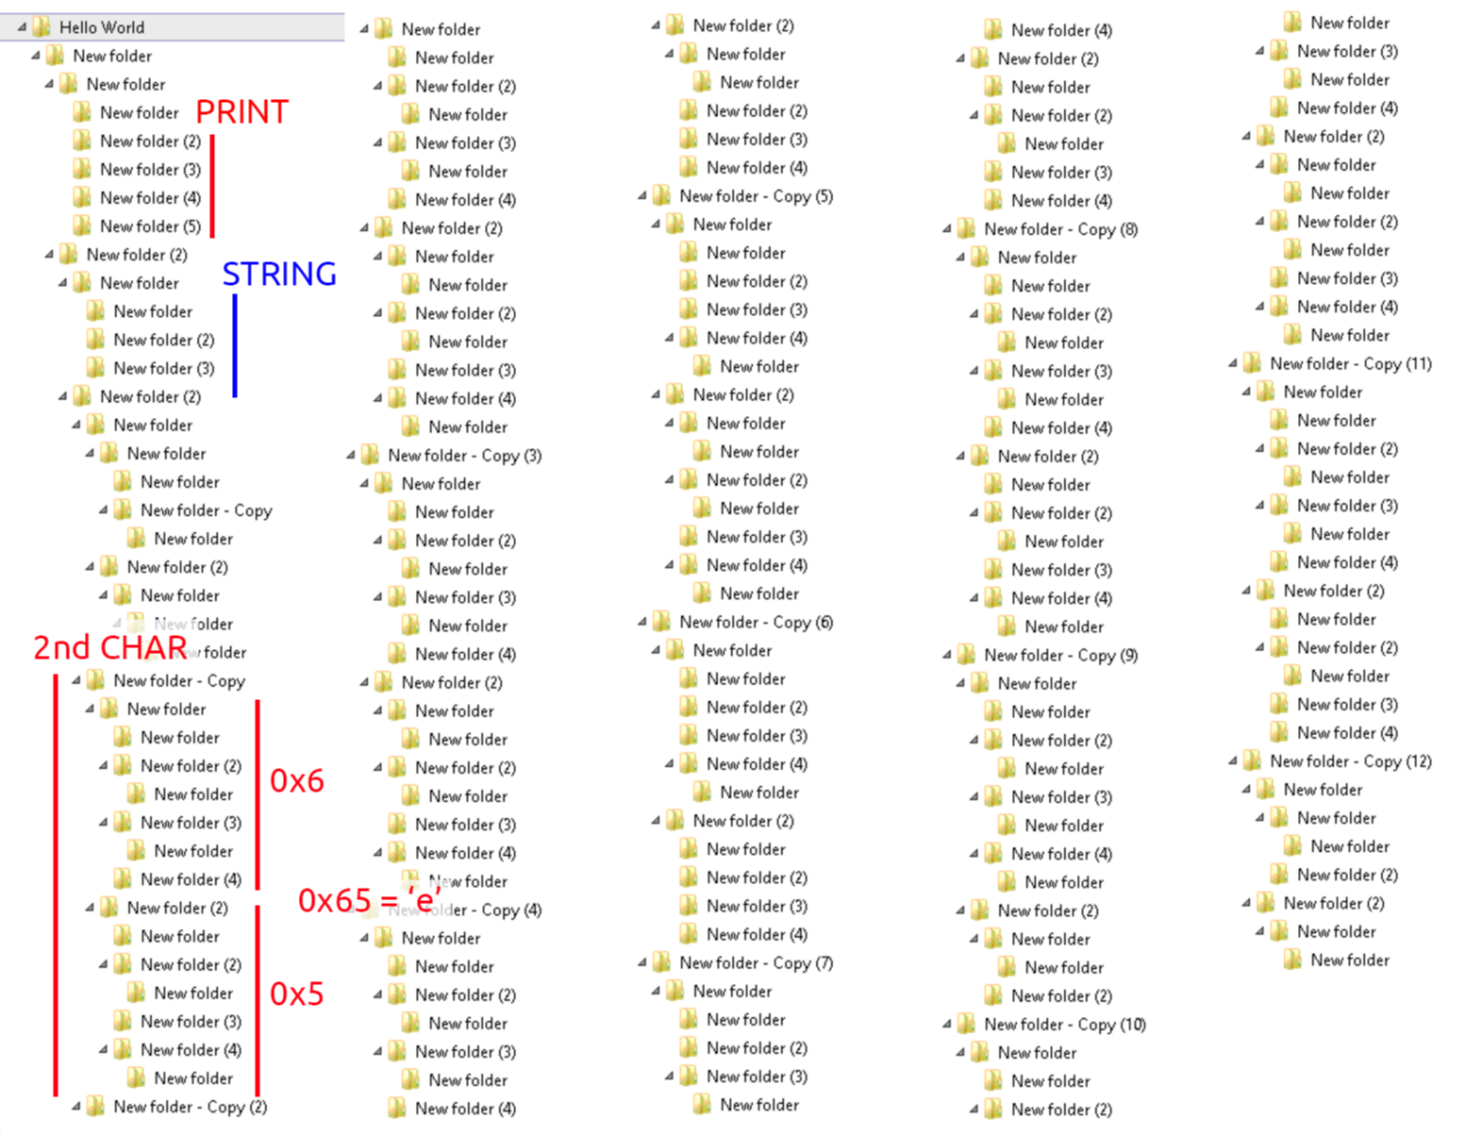
\includegraphics[width=0.8\textwidth,height=\textheight,keepaspectratio,center]{PureFolders_HelloWorld_explained.png}
  \caption{Implementation of the traditional \lstinline{"Hello, world!"} program in the Folders programming language. \citep{temkin_daniel_2015}}
  \label{graphic:folders}
\end{figure}

If hackers subvert our conception of what it means to read, write, execute and understand source code, so do code poems. They are the complementary opposite of such material investigations, arguing rather for the human expressiveness of programming languages. Here, the function is not effective—what actions does programming enable—but useful as it enables new, personal understandings of concepts rendered through programming—what thoughts does the program text enable.

The use of programming languages for poetic purposes (such as \ref{code:black_perl} or \ref{code:self_inspect}) provides a reconciliation of machine execution with human interpretation. Here, the technical environment provides a requirement of syntactical and operational function, while the social environment provides a frame of understanding, reliant on the intention of the writer, of the reader, or of both.

Software can hardly be separated from what it does, and yet cases do exist in order to focus on under-examined aspects of how an artefact is traditionally thought, subverting a naïve understanding of function. In architecture, particular structures do escape expected functional assessments in order to provide new understandings and new possibility, as in the construction of Renaissance follies (displaying symbolic value) or the modern pavillion (displaying technical prowess). Neither of these constructions abide by the traditional function of  architecture (sustaining and sheltering life) but, precisely, these are exceptions confirming the rule, and these extreme examples also help to highlight the default, expected standard, often taken for granted.

We have shown both the variety and necessity of functions in the aesthetic judgment of program texts, stem from their nature as technical artefacts, but also rely on social environments for a program text's primary function to be considered. Furthermore, we have shown that such function is not just material, in the sense of what technology can help us do, but most importantly epistemological, in the sense of what the technology can help us think about, whether a problem domain, a skill, or a feeling. We now conclude this chapter by extending from source code aesthetics into other domains of crafted objects in order to suggest some perspectives on function and aesthetics and how they relate to ethics.

\subsection{Aesthetic and ethical value in program texts}
\label{subsec:aesthetic-ethic-program-texts}

The function of aesthetics in source code is thus an epistemological one, in which particular formal configurations act as a guide towards knowledge of the program's contents, either as a a heuristic from the writer's perspective, or as a cognitive scaffolding from the reader's perspective. Furthermore, its existence as a technical object also implies an existence which can rely both the writer's intent and the reader's use. As intermediary objects, program texts thus possess an ethical dimension, insofar as they need to consider both oneself and the other in the making of decisions resulting in a positively-valued result.

One of the specificities of program texts is that they are collaborative and open-ended, particularly in the open-source movement, which tends to make all program texts writerly texts. Since the audience can become the creator of modified functional technical systems, expressive devices also act as communicative devices, and thus take on a relational dimension. The program text acts as a bridge between the intent of the ideal version of the software, the reality of executing hardware, and the mental spaces constructed by readers and writers. Concluding in the \emph{Languages of Art}, Goodman develops on the relationship between art and understanding, as he compares an artistic attitude, involving an aesthetic experience, with a scientific one:

\begin{quote}
  The difference between art and science is is not that between feeling and fact, intuition and inference, delight and deliberation, synthesis and analysis, sensation and cerebration, concreteness and abstraction, passion and action, mediacy and immediacy, or truth and beauty, but rather a difference in domination of certain specific characteristics of symbols. \citep{goodman_languages_1976}.
\end{quote}

As a crafted technical artifact borrowing from the characteristics of natural language symbol system, and executed by the machine, source code as a medium occupies a hybrid place between art and science. With a genealogy rooted in hard sciences, and with an ontological nature of functionality, it always involves the concept of correctness, a correctness which is always verified through execution. On the other side, the complexity of the computational systems being described, and the uniqueness of the syntax and semantics offered by the medium of source code that is a programming language, require a certain amount of expressiveness found in the use of metaphors to represent concepts from both the problem domain, and from computation itself. Stil, this exchange of knowledge takes place most often between two subjectivities: the writer and the reader.

Writing is, in the moment of its doing, a mostly personal act. When a programmer writes some source code, they do so in a somewhat intimate manner: the only functional judges are onself and the machine, while the only aesthetic judge is oneself. Criteria for aesthetic judgment, at this point, include three axes: the accuracy of the action performed once the program is executed, the ability of the program text to express the concept that is being implemented, and the adequacy of this formal arrangement with the problem at hand—that is, the idiomaticity and elegance of the program text as a solution. Indeed, functional entities appear graceful when they are free of features that are extraneous, or irrelevant in relation to their function. This translation of function into appearance in turn depends on the complementary position: reading source code.

Once a program text is written—that is, once a computational representation of the world has been given textual form—the process of reading introduces new constraints for an aesthetic judgment. Reading a program text involves a process of decrypting the realized adequacy between intent, form and function. This amounts to identifying the semantic affordances, under the form of structure, syntax and vocabulary used by the writer(s) to communicate the ideal action of the program. We put here a particular emphasis on the relationality of such expression. The position of the reader always involves an otherness with respect to the position of the writer. Providing an aesthetic judgment from a reader's perspective thus involves establishing the elegance, fitness, and interest of a certain piece of source code, in accordance with the writer's judgment; because the program text is interpreted by a mechanical third-party, the computer, its value is not exclusively decided by subjective perspectives, and it therefore gains in objectivity. Bruce McLennan writes about this objective component of aesthetics in software engineering, as a way to harmonize the endeavours of the different individuals involved in creative work, from practical construction to the devising of new ideas\footnote{"\emph{Like cathedrals and scientific theories, large software projects are the result of the efforts of many people, and aesthetic standards provide criteria by which individual contributions can be objectively evaluated}" \citep{schummer_aesthetic_2009}}.

This particular relational stance relates to Gerald Weinberg's conception of \emph{egoless programming} \citep{weinberg_psychology_1998}. Considering the practices of professional software developers, Weinberg observes that too much ego lead to non-functional software, as one could not benefit from an external readership in order to weed out mistakes and bugs. One of the ways code can be found to be of good quality is through the giving up of personal ownership for a more collective one. This has first an immediate functional effect, by providing additional layers of quality assurance through the perspectives of everyone which contributes to the program text, directly, or indirectly. It also has an aesthetic consequence, in the form of programming style.

As mentioned in \ref{subsec:style-idioms-programming}, programming style in its individualistic conception is frowned upon, as style should be understood as a collective agreement of ways of doing things. Marielle Macé, in her study of style as a form of life, considers that style is a negotiation between personal and collective ways of being, as an agreement on what matters and on how it should be done\footnote{"\emph{Le « comment » comme lieu d'émergence des valeurs, lieu de querelle sur ce qui compte, lieu d'engagement sur ce qui nous divise et ce qui nous relie. . . C'est la question éthique et politique qui s'ouvre ici, dans sa force d'appel et son indécision fondamentale, celle d'une vie qui est toujours à faire, à débattre, et qui se fonde sur nos différends. Car les manières du vivre n'assument pas un sens ou une valeur a priori ; elles sont le sens et la valeur qu'il y a à faire."} \citep{mace_styles_2016}}. As she considers style as a way of appearing, a way of doing and a way of inhabiting an environment. This last point ties back to the notion of habitability mention in \ref{subsubsec:compression-habitability}. Aesthetics in programming, as a positively valued manifestation at the level of the sense and at the level of the intellect involves a form of transpersonal activity and ties back to a moral virtue of providing habitable spaces. An aesthetically pleasing program text in which one feels at ease to operate, and thus abides by a collective notion of style.

All source code aesthetics relate to a certain conception of function, involving technical achievement and interpersonal existence. An aesthetic judgment of a program text is, in this understanding, the judgment of the perceptible manifestations in source codes allowing for the comprehension of a technical achievement according to contextual standards. These manifestations are therefore not just expressive (personal), but primarily communicative (interpersonal), aiming at the transmission of concepts from one individual through the use of machine syntax through the dual lens of human-machine semantics. Indeed, code that is neither functioning for the machine, nor meaningful for a human holds the least possible value amongst practitioners.

In the overwhelming majority of cases of program texts, the expectation is to understand. Writing aesthetically pleasing code is to write code that engages cognitively its reader, whether explicitly for software developers, pedagogically for scientists, adversely for hackers and metaphorically for poets. This engagement, in turn, supposes an acknowledgement from the writer of the reader. The recognition of the existence of the other as a reader and co-author, implies an acknowledgement as a generalized other in the sense that anyone can theoretically read and modified code, but also as a specificied other, in the sense that the other possesses a particular set of skills, knowledge, habits and practices stemming from the diversity of programming communities. This stance, between general and particular, is one that shows the ethical component of an aesthetic practice: recognizing both the similarity and the difference in the other, and communicating with a peer through specific symbol systems.

\spacer

In conclusion, this chapter has argued first that programming languages provide a socio-technical linguistic environment for the writing of program texts. Acting first as an interface to the computer, programming languages, without overly-determining the practice of programmers or the content of what is being programming, nonetheless influence how it can be said, through idiosyncracies and stylistic devices. This has established the idiosyncratic status of source code as a medium, and its existence between technical and social, expressive and communicative, individual and collaborative.

We then presented a framework for aesthetics of source code, through the dual lense of semantic compression and spatial navigation. To do so, we started from a layer-based approach to the points in which aesthetic decisions can take place in source code—that is, across structure, syntax and vocabulary. Broadening this approach, we then showed how these different levels involve an engagement with semantic layers: between the human reader, the machine reader and the problem domain. The minimizing of syntax while best representing the different concepts involved at these different layers results in semantic compression. A source code with aesthetic value is one which balances syntactic techniques, structural organization and metaphorical choices in order to communicate a socio-technical intent of a functional artefact. In turn, semantic compression supports the shifts from different scales or perspectives the engaged programmer needs to operate as she navigates through her non-linear exploration of a program text.

We concluded this study on the relationship between function and the aesthetic judgment of source code by showing how aesthetic writing involves a certain conception of ethics. Not only is the function of aesthetics in source code is epistemological, in that it enables the acquisition of knowledge, but program texts also involve a tight intertwining  between writer and reader. What must be communicated then is not just what the program does, but how it does it within a given socio-technical context. As we reconsidered the status of style in programming as a transpersonal way of doing, this allowed us to qualify source code aesthetics not as a primarily individual endeavour but moreso as a way of acknowledging the other.